
\chapter{涨落与非平衡统计力学}

在本课程中，我们主要关注各类物理量的统计平均值的计算；这些平均值以高度精确的方式，反映了在给定系统处于平衡状态时，通过相关测量所预期得到的结果。然而，这些平均值仍会存在偏离或围绕其平均值的波动。尽管这些波动通常很小，但出于多种原因，对其研究具有重要的物理意义。

首先，通过对这类波动的研究，我们能够构建一套数学框架，借助该框架，可以对各种物理情境下相关波动的幅度进行估算。毫不意外的是，我们发现：在单相系统中，这些波动在热力学上几乎可以忽略不计，但在多相系统中却可能变得极为重要，尤其是在临界点附近。在后一种情况下，系统中的分子之间会呈现出相当高的空间相关性，而这种相关性又会引发诸如临界乳光等现象。

其次，它为理解一类归于``布朗运动''范畴的现象提供了一个天然的框架；这些现象将流体系统的流动性、扩散系数等属性，通过所谓的爱因斯坦关系，与温度联系起来。布朗运动的机制对于阐明并从某种意义上解答这样一个问题至关重要：即``一个并非处于平衡状态的物理系统，究竟如何最终趋向于达到这样的平衡状态？''而``一个已经处于平衡状态的物理系统，则会持续保持在该状态之中。''

第三，对波动随时间变化的研究，催生了若干``相关函数''的概念，这些函数在关联系统耗散特性------例如流体的粘性阻力或导体的电电阻------与系统处于平衡状态下的微观特性之间发挥着至关重要的作用；这种关系（一方面涉及不可逆过程，另一方面则与平衡性质相互关联）便体现在所谓的``涨落-耗散定理''之中。与此同时，通过对波动``频率谱''的研究------该频谱通过维纳与辛钦基本定理与时间依赖的相关函数相联系------对于评估电气电路中所遇到的``噪声''，以及电磁信号的传输，都具有重要的价值。

\section{平衡热力学涨落}

我们首先推导出某一给定物理系统中若干基本热力学量波动的概率分布律；随后，借助该定律，可以以简便的方式计算这些量的均方波动。我们假设，所给系统可被称作1，嵌入于一个可被称作2的热库之中，从而在两者之间能够实现能量与体积的相互交换；当然，整体能量\(E\)和整体体积\(V\)应保持恒定。为方便起见，我们在此不考虑粒子的交换，因此，数\(N_{1}\)和\(N_{2}\)将各自保持不变。系统的能量\(\overline{E}_{1}\)和\(\overline{E}_{2}\)，以及系统的体积\(\overline{V}_{1}\)和\(\overline{V}_{2}\)，必须满足这样的条件：复合系统\((1+2)\)的1部分和2部分具有共同的温度\(T^{*}\)和共同的压力\(P^{*}\)；请参阅第1.2节和第1.3节，尤其是\autoref{eq:1.3.6}。当然，在平衡状态下，复合系统的熵将达到其最大值；而在任何其他状态------例如那些存在波动的状态------其熵都必然低于这一最大值。若\(\Delta S\)表示复合系统熵与平衡态熵\(S_{0}\)之间的偏差，则

\begin{equation}\tag{15.1.1}\label{eq:15.1.1}
\Delta S \equiv S - S _ { 0 } = k \ln \Omega _ { f } - k \ln \Omega _ { 0 } ,
\end{equation}

其中\(\Omega_{f}\)（或\(\Omega_{0}\)）表示系统\((1+2)\)在存在（或不存在）偏离平衡态的波动时所具有的不同微观状态的数量；请参阅\autoref{eq:1.2.6}。因此，所提出的波动确实发生的概率可由下式给出：

\begin{equation}\tag{15.1.2}\label{eq:15.1.2}
p \propto \Omega _ { f } \propto \exp ( \Delta S / k ) ;
\end{equation}

参见第3.1节，尤其是\autoref{eq:3.1.3}。从其他热力学量的角度来看，我们可以写成

\begin{equation}\tag{15.1.3}\label{eq:15.1.3}
\Delta S = \Delta S _ { 1 } + \Delta S _ { 2 } = \Delta S _ { 1 } + \int _ { 0 } ^{f} \frac { d E _ { 2 } + P _ { 2 } d V _ { 2 } } { T _ { 2 } } ;
\end{equation}

?????????\(P_{2}\)???\(T_{2}\)??????????????????????????1???????????????????2??????????????????????\(P_{2}\)?\(T_{2}\)????????\(P^{*}\)?\(T^{*}\)????????\(dE_{2}\)?\(dV_{2}\)???????\(-dE_{1}\)?\(-dV_{1}\)????\autoref{eq:15.1.3}??

\begin{equation}\tag{15.1.4}\label{eq:15.1.4}
\Delta S = \Delta S _ { 1 } - ( \Delta E _ { 1 } + P ^{*} \Delta V _ { 1 } ) / T ^{*} .
\end{equation}

????\autoref{eq:15.1.2}?????

\begin{equation}\tag{15.1.5}\label{eq:15.1.5}
p \propto \exp \{ - ( \Delta E _ { 1 } - T ^{*} \Delta S _ { 1 } + P ^{*} \Delta V _ { 1 } ) / k T ^{*} \} .
\end{equation}

显然，公式（5）所描述的概率分布律在任何方面都不依赖于该系统所处的储层本身的特殊性。因此，公式（5）同样适用于在统计系综中达到平衡的系统------或者说，它也适用于给定系统本身中的任意宏观部分。由此，我们可以将符号 \(\Delta E_{1}\)、\(\Delta S_{1}\) 和 \(\Delta V_{1}\) 中的后缀 1 以及符号 \(P^{*}\) 和 \(T^{*}\) 中的星号去掉，改写为

\begin{equation}\tag{15.1.6}\label{eq:15.1.6}
p \propto \exp \{ - ( \Delta E - T \Delta S + P \Delta V ) / k T \} .
\end{equation}

在大多数情况下，这些波动的幅度极其微小；因此，量 \(\Delta E\) 可以围绕平衡值 \((\Delta E)_0 = 0\) 进行泰勒展开，其结果为

\begin{equation}\tag{15.1.7}\label{eq:15.1.7}
\begin{array}{rl} & { \Delta E = \left( \frac { \partial E } { \partial S } \right) _ { 0 } \Delta S + \left( \frac { \partial E } { \partial V } \right) _ { 0 } \Delta V } \\& {  + \frac { 1 } { 2 } \left[ \left( \frac { \partial ^{2} E } { \partial S ^{2} } \right) _ { 0 } ( \Delta S ) ^{2} + 2 \left( \frac { \partial ^{2} E } { \partial S \partial V } \right) _ { 0 } \Delta S \Delta V + \left( \frac { \partial ^{2} E } { \partial V ^{2} } \right) _ { 0 } ( \Delta V ) ^{2} \right] + \cdots } \end{array}
\end{equation}

将式（7）代入式（6），仅保留至二阶项，我们得到

\begin{equation}\tag{15.1.8}\label{eq:15.1.8}
p \propto \exp \{ - ( \Delta T \Delta S - \Delta P \Delta V ) / 2 k T \} ;
\end{equation}

在此，我们利用了以下关系

\begin{equation}\tag{15.1.9}\label{eq:15.1.9}
\left( \frac { \partial E } { \partial S } \right) _ { 0 } = T ,  \left( \frac { \partial E } { \partial V } \right) _ { 0 } = - P ,
\end{equation}

并且注意到，式（7）中括号内的表达式与

\begin{equation}\tag{15.1.10}\label{eq:15.1.10}
\Delta \left( \frac { \partial E } { \partial S } \right) _ { 0 } \Delta S + \Delta \left( \frac { \partial E } { \partial V } \right) _ { 0 } \Delta V = \Delta T \Delta S - \Delta P \Delta V .
\end{equation}

借助式（8），各种物理量的均方波动以及不同波动之间的统计相关性均可轻松计算。不过，我们注意到，在这个公式中出现的四个 \(\Delta\) 项中，只有两个可以独立选取；另外两个则必须充当``推导出的量''。例如，如果我们选择 \(\Delta T\) 和 \(\Delta V\) 作为独立变量，那么 \(\Delta S\) 和 \(\Delta P\) 就可以表示为

\begin{equation}\tag{15.1.11}\label{eq:15.1.11}
\Delta S = \left( \frac { \partial S } { \partial T } \right) _ { V } \Delta T + \left( \frac { \partial S } { \partial V } \right) _ { T } \Delta V = \frac { C _ { V } } { T } \Delta T + \left( \frac { \partial P } { \partial T } \right) _ { V } \Delta V
\end{equation}

并

\begin{equation}\tag{15.1.12}\label{eq:15.1.12}
\Delta P = \left( \frac { \partial P } { \partial T } \right) _ { V } \Delta T + \left( \frac { \partial P } { \partial V } \right) _ { T } \Delta V = \left( \frac { \partial P } { \partial T } \right) _ { V } \Delta T - \frac { 1 } { \kappa _ { T } V } \Delta V ,
\end{equation}

\(\kappa_{T}\) 是系统的等温压缩率。将式（11）和式（12）代入式（8），我们得到

\begin{equation}\tag{15.1.13}\label{eq:15.1.13}
p \propto \exp \left\{ - \frac { C _ { V } } { 2 k T ^{2} } ( \Delta T ) ^{2} - \frac { 1 } { 2 k T \kappa _ { T } V } ( \Delta V ) ^{2} \right\} ,
\end{equation}

这表明 \(T\) 和 \(V\) 的波动在统计上是相互独立的、呈高斯分布的！快速查看式（13），我们便能得到如下结果

\begin{equation}\tag{15.1.14}\label{eq:15.1.14}
\overline { { ( \Delta T ) ^{2} } } = \frac { k T ^{2} } { C _ { V } } ,  \overline { { ( \Delta V ) ^{2} } } = k T \kappa _ { T } V ,
\end{equation}

而

\begin{equation}\tag{15.1.15}\label{eq:15.1.15}
\overline { { ( \Delta T \Delta V ) } } = 0 .
\end{equation}

同样地，如果我们选择 \(\Delta S\) 和 \(\Delta P\) 作为独立变量，我们便会得出分布律

\begin{equation}\tag{15.1.16}\label{eq:15.1.16}
p \propto \exp \left\{ - \frac { 1 } { 2 k C _ { P } } ( \Delta S ) ^{2} - \frac { \kappa _ { S } V } { 2 k T } ( \Delta P ) ^{2} \right\} ,
\end{equation}

该分布律给出

\begin{equation}\tag{15.1.17}\label{eq:15.1.17}
\overline { { ( \Delta S ) ^{2} } } = k C _ { P } ,  \overline { { ( \Delta P ) ^{2} } } = \frac { k T } { \kappa _ { S } V } ,
\end{equation}

而

\begin{equation}\tag{15.1.18}\label{eq:15.1.18}
\overline { { ( \Delta S \Delta P ) } } = 0 ;
\end{equation}

在此，\(\kappa_{S}\) 表示系统的绝热压缩率。

我们注意到，一般来说，广义量的均方波动与系统大小成正比，而狭义量的均方波动则与系统大小成反比；在两种情况下，任意量的相对均方波动都与系统大小的平方根成反比。因此，除了在临界区域等特定情形下之外，正常的波动在热力学上几乎可以忽略不计。但这并不意味着波动完全与系统中发生的物理现象无关；事实上，正如后续章节所将要展示的那样，微观层面的波动本身对于系统在宏观层面所展现的诸多性质而言，具有根本性的意义！

借助上述结果，我们可以对系统的能量均方波动进行计算。以 \(T\) 和 \(V\) 为独立变量，我们有

\begin{equation}\tag{15.1.19}\label{eq:15.1.19}
\Delta E = \left( { \frac { \partial E } { \partial T } } \right) _ { V } \Delta T + \left( { \frac { \partial E } { \partial V } } \right) _ { T } \Delta V .
\end{equation}

将该表达式平方并取平均值时，同时牢记公式（14），我们得到

\begin{equation}\tag{15.1.20}\label{eq:15.1.20}
\begin{array}{r} { \overline { { ( \Delta E ) ^{2} } } = k T ^{2} C _ { V } + k T \kappa _ { T } V \left\{ \left( \frac { \partial E } { \partial V } \right) _ { T } \right\} ^{2} } \\{ = k T ^{2} C _ { V } + k T \kappa _ { T } \left( \frac { N ^{2} } { V } \right) \left\{ \left( \frac { \partial E } { \partial N } \right) _ { T } \right\} ^{2} . } \end{array}
\end{equation}

现在，前几段中推导出的结果，只要给定系统中的某个宏观子系统内粒子数保持不变，便可用来确定该系统中各物理量的波动。因此，可利用公式（14b）来推导出该子系统中变量 \(v\)（单位粒子体积）和变量 \(n\)（粒子密度）的均方波动表达式。我们很容易得出

\begin{equation}\tag{15.1.21}\label{eq:15.1.21}
\overline { { ( \Delta v ) ^{2} } } = k T \kappa _ { T } V / N ^{2} ,  \overline { { ( \Delta n ) ^{2} } } = \frac { 1 } { v ^{4} } \overline { { ( \Delta v ) ^{2} } } = k T \kappa _ { T } N ^{2} / V ^{3} ;
\end{equation}

值得注意的是，此处得出的最后一个结果与基于大canonical系综推导出的公式（4.5.7）完全一致。稍加思索便会发现，这一结果同样适用于一个体积 \(V\) 固定、粒子数 \(N\) 变化的子系统。此时，\(N\) 的均方波动可表示为

\begin{equation}\tag{15.1.22}\label{eq:15.1.22}
\overline { { ( \Delta N ) ^{2} } } = V ^{2} \overline { { ( \Delta n ) ^{2} } } = k T \kappa _ { T } N ^{2} / V .
\end{equation}

将（20）代入（18），我们再次得到了大canonical系综关于 \(\overline{(\Delta E)^2}\) 的结果，即

\begin{equation}\tag{15.1.23}\label{eq:15.1.23}
\overline { { ( \Delta E ) ^{2} } } = k T ^{2} C _ { V } + \overline { { ( \Delta N ) ^{2} } } \{ ( \partial E / \partial N ) _ { T } \} ^{2} ,
\end{equation}

如同公式（4.5.14）所示。

顺便指出，公式（21）的第一部分，正是指在 \(N\) 和 \(V\) 都固定的情况下，某子系统能量 \(E\) 的均方波动------这与我们在canonical系综 \((N,V,T)\) 中所采用的方式完全相同。反之，若我们假设能量 \(E\) 固定，则子系统的温度将会发生波动，而量 \(\Delta T\) 的均方值将由 \((kT^2C_V)\) 除以子系统热容的平方所得。因此，最终结果为 \((kT^2/C_V)\)，这与公式（14a）中的结果完全一致。

\section{爱因斯坦-斯莫卢霍夫斯基的布朗运动理论}\label{ux7231ux56e0ux65afux5766-ux65afux83abux5362ux970dux592bux65afux57faux7684ux5e03ux6717ux8fd0ux52a8ux7406ux8bba}

``布朗运动''这一术语源自植物学家罗伯特·布朗。1828年，他在显微镜下对某种植物的微小花粉颗粒进行了细致的观察。用他自己的话说：``在检查那些浸没在水中的颗粒形态时，我注意到\ldots\ldots{}''

其中许多颗粒显然在不断运动。这些运动方式让我确信\ldots\ldots 它们既非源于流体中的电流，也非因流体的缓慢蒸发所致，而是完全属于颗粒本身。''如今我们已知，这种运动的真正来源在于布朗粒子所遭受的、持续且或多或少随机的碰撞与轰击------而这些颗粒（或者说，任何胶体悬浮液）通常都由周围流体的分子所``赋予''其名称。正是爱因斯坦在多篇论文中（自1905年起）首次基于所谓的``随机游走问题''，对布朗运动进行了严谨的理论分析，并由此确立了这一现象不可逆性与分子涨落机制之间深远的联系。

为了阐明爱因斯坦研究方法的核心要义，我们先从一维情形入手。设 \(x(t)\) 表示布朗粒子在时间 \(t\) 时的位置，假设该粒子在 \(t=0\) 时的位置恰好为 \(x=0\)。为简化问题，我们假定每次分子撞击（平均而言，每经过一段时长 \(\tau^{*}\) 后发生一次）都会使粒子沿 \(x\) 轴正向或负向跳动一个（大小恒定的）距离 \(l\)。自然地，我们认为 \(\Delta x=+l\) 和 \(\Delta x=-l\) 这两种可能发生的概率是相等的；尽管稍显不那么自然，我们也可以认为，布朗粒子随后的多次撞击及其随之而来的连续跳跃彼此之间并无相关性。因此，粒子在时间 \(t\) 时位于点 \(x\) 的概率，等于在一系列 \(n=(t/\tau^{*})\) 次连续跳跃中，粒子在 \(x\) 轴正向的跳跃次数比在负向多 \(m=(x/l)\) 次------也就是说，粒子在正向方向上完成了 \(\frac{1}{2}(n+m)\) 次跳跃，在负向方向上完成了 \(\frac{1}{2}(n-m)\) 次跳跃。所需的概率则由二项式表达式给出：

\begin{equation}\tag{15.2.1}\label{eq:15.2.1}
p _ { n } ( m ) \equiv \frac { n ! } { \left\{ \frac { 1 } { 2 } ( n + m ) \right\} ! \left\{ \frac { 1 } { 2 } ( n - m ) \right\} ! } \left( \frac { 1 } { 2 } \right) ^{n} ,
\end{equation}

结果是，

\begin{equation}\tag{15.2.2}\label{eq:15.2.2}
{ \overline { { m } } } = 0  { \mathrm { a n d } }  { \overline { { m ^{2} } } } = n .
\end{equation}

因此，当 \(t \gg \tau^{*}\) 时，粒子的净位移为

\begin{equation}\tag{15.2.3}\label{eq:15.2.3}
\overline { { x ( t ) } } = 0  \mathrm { a n d }  \overline { { x ^{2} ( t ) } } = l ^{2} \, \frac { t } { \tau ^{*} } \propto t ^{1} .
\end{equation}

相应地，粒子的均方根位移与所经历的时间平方根成正比：

\begin{equation}\tag{15.2.4}\label{eq:15.2.4}
x _ { \mathrm { r . m . s . } } = \sqrt { \left( \overline { { x ^{2} ( t ) } } \right) } = l \sqrt { ( t / \tau ^{*} ) } \propto t ^{1 / 2} .
\end{equation}

值得注意的是，布朗粒子的``净''整体位移与基本步数总和的平方根成正比，这正是一个典型的结论。

步长的随机性在自然界中以多种多样的现象形式展现出来。相比之下，如果各步骤之间完全连贯一致（或者若运动在时间间隔 \(t\) 内完全可预测且可逆），² 则布朗粒子的净位移将与 \(t^{1}\) 成正比。

斯莫卢霍夫斯基于 1906 年提出的布朗运动问题研究方法，本质上与爱因斯坦的方法如出一辙；二者的主要差异在于数学推导过程。斯莫卢霍夫斯基引入了概率函数 \(p_{n}(x_{0}|x)\)，该函数表示``在经过一系列 \(n\) 个步骤后，初始位于点 \(x_{0}\) 的布朗粒子到达点 \(x\) 的概率''；此处的数字 \(x\) 表示布朗粒子沿小步长度所行进的距离。显然，

\begin{equation}\tag{15.2.5}\label{eq:15.2.5}
p _ { n } ( x _ { 0 } | x ) = \sum _ { z = - \infty } ^{\infty} p _ { n - 1 } ( x _ { 0 } | z ) p _ { 1 } ( z | x )  ( n \geq 1 ) ;
\end{equation}

此外，由于每次一步都同样有可能使粒子向右移动，或向左移动，

\begin{equation}\tag{15.2.6}\label{eq:15.2.6}
p _ { 1 } ( z | x ) = \frac { 1 } { 2 } \delta _ { z , x - 1 } + \frac { 1 } { 2 } \delta _ { z , x + 1 } ,
\end{equation}

而

\begin{equation}\tag{15.2.7}\label{eq:15.2.7}
p _ { 0 } ( z | x ) = \delta _ { z , x } .
\end{equation}

\autoref{eq:15.2.5}???????????????????????????????? \(Q_{n}(\xi)\)??

\begin{equation}\tag{15.2.8}\label{eq:15.2.8}
Q _ { n } ( \xi ) = \sum _ { x = - \infty } ^{\infty} p _ { n } ( x _ { 0 } | x ) \xi ^{x - x _ { 0} } ,
\end{equation}

由此可以推导出

\begin{equation}\tag{15.2.9}\label{eq:15.2.9}
Q _ { 0 } ( \xi ) = \sum _ { x = - \infty } ^{\infty} p _ { 0 } ( x _ { 0 } | x ) \xi ^{x - x _ { 0} } = \sum _ { x = - \infty } ^{\infty} \delta _ { x _ { 0 } , x } \xi ^{x - x _ { 0} } = 1 .
\end{equation}

将 (6) 代入 (5)，我们得到

\begin{equation}\tag{15.2.10}\label{eq:15.2.10}
p _ { n } ( x _ { 0 } | x ) = \frac { 1 } { 2 } p _ { n - 1 } ( x _ { 0 } | x - 1 ) + \frac { 1 } { 2 } p _ { n - 1 } ( x _ { 0 } | x + 1 ) .
\end{equation}

? ????????????????????????????????????? \(t\) ?? \(-t\) ??????????????????????????????????????????????????????????????????????????????????????????????????\autoref{eq:15.2.19}??????????????????????????

将 (10) 乘以 \(\xi^{x-x_0}\)，并对其所有 \(x\) 进行求和，我们得到递推关系

\begin{equation}\tag{15.2.11}\label{eq:15.2.11}
Q _ { n } ( \xi ) = \frac { 1 } { 2 } [ \xi + ( 1 / \xi ) ] Q _ { n - 1 } ( \xi ) ,
\end{equation}

因此，通过迭代计算，

\begin{equation}\tag{15.2.12}\label{eq:15.2.12}
Q _ { n } ( \xi ) = \left\{ \frac { 1 } { 2 } [ \xi + ( 1 / \xi ) ] \right\} ^{n} Q _ { 0 } ( \xi ) = ( 1 / 2 ) ^{n} [ \xi + ( 1 / \xi ) ] ^{n} .
\end{equation}

将此表达式按二项式展开，并将结果与 (8) 进行比较，我们得到

\begin{equation}\tag{15.2.13}\label{eq:15.2.13}
\begin{array}{rlr} & { } & { p _ { n } ( x _ { 0 } | x ) = \left( \frac { 1 } { 2 } \right) ^{n} \frac { n ! } { \{ \frac { 1 } { 2 } ( n + x - x _ { 0 } ) \} ! \{ \frac { 1 } { 2 } ( n - x + x _ { 0 } ) \} ! }  \mathrm { f o r } \ | x - x _ { 0 } | \leq n } \\& { } & { 0         \mathrm { f o r } \ | x - x _ { 0 } | > n . } \end{array}
\end{equation}

将 \((x-x_{0})\) 与 \(m\) 对应起来，我们发现这一结果与我们先前得出的结论 (1) 完全一致。³ 因此，从斯莫卢霍夫斯基方法得出的任何结论，都将与从爱因斯坦方法得出的结论完全相同。

为了获得 \(p_{n}(m)\) 函数的渐近形式，我们对 (1) 中的阶乘应用斯特林公式 \(n! \approx (2\pi n)^{1/2}(n/e)^{n}\)，其结果是

\begin{equation}\tag{15.2.14}\label{eq:15.2.14}
\begin{array}{r} { \ln p _ { n } ( m ) \approx \left( n + \frac { 1 } { 2 } \right) \ln n - \frac { 1 } { 2 } ( n + m + 1 ) \ln \left\{ \frac { 1 } { 2 } ( n + m ) \right\} } \\{ - \frac { 1 } { 2 } ( n - m + 1 ) \ln \left\{ \frac { 1 } { 2 } ( n - m ) \right\} - n \ln 2 - \frac { 1 } { 2 } \ln ( 2 \pi ) . } \end{array}
\end{equation}

对于 \(m \ll n\)（通常情况下这一条件成立，因为 \(\overline{m} = 0\)，且 \(m_{\text{r.m.s.}} = n^{1/2}\)，而 \(n \gg 1\)），我们得到

\begin{equation}\tag{15.2.15}\label{eq:15.2.15}
p _ { n } ( m ) \approx \frac { 2 } { \sqrt { ( 2 \pi n ) } } \exp ( - m ^{2} / 2 n ) .
\end{equation}

? \(x\) ?????????? \(p_{n}(m) \equiv 0\)??? \(m\) ???????????\autoref{eq:15.2.14}??\(\Delta m = 2\) ?? 1??????????????????

\begin{equation}\tag{15.2.16}\label{eq:15.2.16}
p ( x ) d x = { \frac { d x } { \sqrt { ( 4 \pi D t ) } } } \exp \left( - { \frac { x ^{2} } { 4 D t } } \right) ,
\end{equation}

其中

\begin{equation}\tag{15.2.17}\label{eq:15.2.17}
D = l ^{2} / 2 \tau ^{*} .
\end{equation}

³ 人们很容易意识到这样一个额外的事实：如果 \(n\) 是偶数，则对于奇数 \(m\)，\(p_{n}(m) \equiv 0\)；而如果 \(n\) 是奇数，则对于偶数 \(m\)，\(p_{n}(m) \equiv 0\)。

?????????????? \(D\) ???????????????\autoref{eq:15.2.16}???????? \(l\) ? \(\tau^*\) ?????????????????????????????????????????????????????????????????????????????????????????????????????????????????????? Lee?Sears ? Turcotte?1963????????????? 2 ???????? \(\Delta x\) ? 403 ?????????????

\begin{longtable}[]{@{}l@{}}
\toprule\noalign{}
位移 \(\Delta x\)，以 μ（即 \(10^{-4}\) 厘米）为单位 \\
\midrule\noalign{}
\endhead
\bottomrule\noalign{}
\endlastfoot
小于 -5.5 \\
在 -5.5 到 -4.5 之间 \\
在 -4.5 到 -3.5 之间 \\
在 -3.5 到 -2.5 之间 \\
在 -2.5 到 -1.5 之间 \\
在 -1.5 到 -0.5 之间 \\
在 -0.5 到 +0.5 之间 \\
在 +0.5 到 +1.5 之间 \\
在 +1.5 到 +2.5 之间 \\
在 +2.5 到 +3.5 之间 \\
在 +3.5 到 +4.5 之间 \\
大于 +4.5 \\
\end{longtable}

在此处，位移的均方值为：\(\overline{(\Delta x)^2} = 2.09 \times 10^{-8}\) 平方厘米。所观察到的频率分布以``块状图''的形式绘制在图 15.1 中。我们在该图中加入了基于观测到的均方位移值的高斯曲线；我们发现，实验数据与理论曲线的拟合程度相当理想。我们还可以在此推导出介质扩散系数的实验值：\(D = (\Delta x)^2/2t = 5.22 \times 10^{-9}\) 平方厘米/秒。4

现在，我们从扩散的角度来研究布朗运动。我们将流体中布朗粒子的数密度记为 \(n(\boldsymbol{r},t)\)，其电流密度则记为 \(\boldsymbol{j}(\boldsymbol{r},t)\{=n(\boldsymbol{r},t)\boldsymbol{v}(\boldsymbol{r},t)\}\)；根据菲克定律，

\begin{equation}\tag{15.2.18}\label{eq:15.2.18}
\begin{array}{r} { \mathbf { j } ( \mathbf { r } , t ) = - D \nabla n ( \mathbf { r } , t ) , } \end{array}
\end{equation}

在下一节中，我们将看到，对于一个球形粒子，扩散系数 \(D\) 可以表示为 \(D = kT / (6\pi\eta a)\)，其中 \(\eta\) 是介质的粘度系数，\(a\) 是布朗粒子的半径。在所研究的案例中，\(T \approx 300\mathrm{K}\)，\(\eta \approx 10^{-2}\) 帕斯卡·秒，\(a \approx 4 \times 10^{-5}\mathrm{cm}\)。将这些数值代入，我们得到玻尔兹曼常数的值：\(k \approx 1.3 \times 10^{-16}\mathrm{erg/K}\)。

\begin{equation}\tag{15.2.17}\label{eq:15.2.17_continuity}
\nabla \cdot \mathbf { j } ( \pmb { r } , t ) + \frac { \partial n ( \pmb { r } , t ) } { \partial t } = 0 .
\end{equation}

将式（17）代入式（18），我们得到了扩散方程

\begin{equation}\tag{15.2.19}\label{eq:15.2.19}
\nabla ^{2} n ( \mathbf { r } , t ) - \frac { 1 } { D } \frac { \partial n ( \mathbf { r } , t ) } { \partial t } = 0 .
\end{equation}

在该方程的各种可能解中，与当前情形相关的解是

\begin{equation}\tag{15.2.20}\label{eq:15.2.20}
n ( \pmb { r } , t ) = \frac { N } { ( 4 \pi D t ) ^{3 / 2} } \exp \left( - \frac { r ^{2} } { 4 D t } \right) ,
\end{equation}

该解具有球对称性，并且已经进行了归一化处理：

\begin{equation}\tag{15.2.21}\label{eq:15.2.21}
\int _ { 0 } ^{\infty} n ( \mathbf { r } , t ) 4 \pi r ^{2} d \mathbf { r } = N ,
\end{equation}

\(N\) 代表完全浸没在流体中的所有（布朗）粒子总数。将（三维）结果式（20）与（一维）结果式（15）进行比较，可以最清晰地揭示出：一方面存在随机游走问题，另一方面又对应着扩散现象。

显然，在上一种方法中，我们考虑的是由 \(N\) 个布朗粒子组成的``整体''在``等效''的物理条件下运动，而非像在随机游走方法中那样，单独考虑单个粒子在某一时间跨度内的运动。因此，此处获得的各类物理量的平均值，本质上属于``整体平均值''；当然，它们必须与先前获得的同一类物理量的长期平均值相一致。

现在，借助于分布式（20），我们得到

\begin{equation}\tag{15.2.22}\label{eq:15.2.22}
\langle r ( t ) \rangle = 0 ;  \langle r ^{2} ( t ) \rangle = \frac { 1 } { N } \int _ { 0 } ^{\infty} n ( r , t ) 4 \pi r ^{4} d r = 6 D t \propto t ^{1} ,
\end{equation}

与我们先前的结果完全一致，即

\begin{equation}\tag{15.2.23}\label{eq:15.2.23}
\overline { { x ( t ) } } = 0 ;  \overline { { x ^{2} ( t ) } } = l ^{2} t / \tau ^{*} = 2 D t \propto t ^{1} .
\end{equation}

因此，最初集中于原点的布朗粒子``集合体''会随着时间的推移而``扩散开来''，其在任意时刻 \(t\) 的扩散性质与程度分别由式（20）和式（22）给出。这一显然不可逆的扩散过程，为我们提供了对集合体中单个粒子统计行为相当清晰的认识。然而，需要牢记的一点是：无论我们将注意力集中在集合体中的单个粒子上，还是将整个集合体作为一个整体来观察，这一现象的最终根源都在于布朗粒子所受到的、来自流体分子的持续且或多或少随机的撞击。换句话说，这一现象的不可逆性，归根结底源于流体分子对布朗粒子施加的随机、波动性力。这又引出了另一套系统性的布朗运动理论------即朗之万理论（1908年）。有关该问题的详细分析，请参阅乌伦贝克与奥恩斯坦（1930年）、钱德拉塞卡（1943年、1949年）、麦克唐纳（1948--1949年）以及沃克斯（1954年）的相关著作。

\section{朗之万理论下的布朗运动}\label{ux6717ux4e4bux4e07ux7406ux8bbaux4e0bux7684ux5e03ux6717ux8fd0ux52a8}

我们考虑最简单的``自由''布朗粒子情形，该粒子被流体环境所包围；假设该粒子处于自由状态，即它不受任何其他力的作用，仅受来自分子碰撞所产生的力的影响。此时，粒子的运动方程将为：

\begin{equation}\tag{15.3.1}\label{eq:15.3.1}
M { \frac { d v } { d t } } = { \mathcal { F } } ( t ) ,
\end{equation}

其中 \(M\) 为粒子质量，\(\boldsymbol{v}(t)\) 为粒子速度，\(\mathcal{F}(t)\) 则为由于粒子受到流体分子撞击而作用于其上的力。朗之万提出，力 \(\mathcal{F}(t)\) 可以写成两部分之和：（一）一个``平均化''的部分，即粒子所经历的粘性阻力，\(-\boldsymbol{v}/B\)；相应地，\(B\) 为系统的迁移率，亦即粒子在单位``外力''作用下所获得的漂移速度。（5）（二）一个``快速波动''的部分 \(F(t)\)，在较长的时间间隔内，

在与特征时间 \(\tau^{*}\) 相比的较短时间内，该部分会趋于零；因此，我们可以将其表示为

\begin{equation}\tag{15.3.2}\label{eq:15.3.2}
M { \frac { d v } { d t } } = - { \frac { v } { B } } + F ( t ) ;  { \overline { { F ( t ) } } } = 0 .
\end{equation}

对式（2）进行集合平均后，我们得到

\begin{equation}\tag{15.3.3}\label{eq:15.3.3}
M \frac { d } { d t } \langle \pmb { v } \rangle = - \frac { 1 } { B } \langle \pmb { v } \rangle ,
\end{equation}

由此可得

\begin{equation}\tag{15.3.4}\label{eq:15.3.4}
\langle v ( t ) \rangle = v ( 0 ) \exp ( - t / \tau )  ( \tau = M B ) .
\end{equation}

因此，粒子的平均漂移速度会以由弛豫时间 \(\tau\) 决定的速率衰减至最终值零。值得注意的是，这一结果正是由流体黏度等耗散特性所支配的现象的典型特征；其结果的不可逆性也显而易见。

将式（2）除以粒子质量，我们得到了瞬时加速度的表达式，即

\begin{equation}\tag{15.3.5}\label{eq:15.3.5}
\frac { d v } { d t } = - \frac { v } { \tau } + A ( t ) ;  \overline { { A ( t ) } } = 0 .
\end{equation}

我们现在将式（5）与粒子的瞬时位置 \(r\) 进行标量积，并对这一乘积取集合平均。在这一过程中，我们利用了以下事实：（i）\(r \cdot v = \frac{1}{2}(dr^2/dt)\)，（ii）\(r \cdot (dv/dt) = \frac{1}{2}(d^2r^2/dt^2) - v^2\)，以及（iii）\(\langle r \cdot A \rangle = 0\)。我们得到

\begin{equation}\tag{15.3.6}\label{eq:15.3.6}
\frac { d ^{2} } { d t ^{2} } \langle r ^{2} \rangle + \frac { 1 } { \tau } \frac { d } { d t } \langle r ^{2} \rangle = 2 \langle v ^{2} \rangle .
\end{equation}

如果布朗运动粒子已经与流体分子达到了热平衡，那么该方程中的 \(\langle v^{2}\rangle\) 可以用其等分能量值 \(3kT/M\) 替代。随后，该方程可轻松进行积分，其结果为

\begin{equation}\tag{15.3.7}\label{eq:15.3.7}
\langle r ^{2} \rangle = \frac { 6 k T \tau ^{2} } { M } \left\{ \frac { t } { \tau } - ( 1 - e ^{- t / \tau} ) \right\} ,
\end{equation}

\^{}\{6\}``对一个集合进行平均''的过程意味着，我们是在想象大量与最初所研究系统相似的系统，并在任意时刻 \(t\) 对这一集合进行平均。由于函数 \(F(t)\) 的本质特性，集合平均值 \(\langle F(t) \rangle\) 在任何时刻都必为零。

\^{}\{7\}之所以如此，是因为我们并没有理由预期布朗运动粒子的位置 \(\boldsymbol{r}(t)\) 与流体分子对其施加的力 \(F(t)\) 之间存在统计相关性；不过，请参阅 Manoliu 和 Kittel（1979）。当然，我们确实预期 \(\boldsymbol{v}(t)\) 与 \(F(t)\) 之间存在相关性；因此，\(\langle \boldsymbol{v} \cdot F \rangle \neq 0\)（详见问题 15.7）。

其中，积分常数的选取方式使得在 \(t=0\) 时，\(\langle r^{2}\rangle\) 及其一阶时间导数均变为零。我们注意到，在 \(t \ll \tau\) 时，

\begin{equation}\tag{15.3.8}\label{eq:15.3.8}
\langle r ^{2} \rangle \simeq \frac { 3 k T } { M } t ^{2} = \langle v ^{2} \rangle t ^{2} ,
\end{equation}

这与可逆的运动方程一致------按照这些方程，我们只需

\begin{equation}\tag{15.3.9}\label{eq:15.3.9}
r = v t .
\end{equation}

另一方面，当 \(t \gg \tau\) 时，

\begin{equation}\tag{15.3.10}\label{eq:15.3.10}
\langle r ^{2} \rangle \simeq \frac { 6 k T \tau } { M } t = ( 6 B k T ) t ,
\end{equation}

这本质上与 Einstein--Smoluchowski 结果（15.2.22）相同；顺便说一下，我们在此得到了一个简单却至关重要的关系：扩散系数 \(D\) 与迁移率 \(B\) 之间的关系，即

\begin{equation}\tag{15.3.11}\label{eq:15.3.11}
D = B k T ,
\end{equation}

这一关系通常被称为 Einstein 关系。

方程（10）的不可逆性不言自明；同样显而易见的是，这一方程本质上源于介质的粘度。此外，Einstein 关系（11），它将扩散系数 \(D\) 与系统的迁移率 \(B\) 相联系，告诉我们：介质粘度（以及扩散现象）的最终来源，正是由流体分子持续不断的运动所引发的随机、波动性力；另请参阅第 15.6 节中的涨落-耗散定理。

在此背景下，若我们考虑一个电荷为 \(e\)、质量为 \(M\) 的粒子，在外加电场强度为 \(E\) 的作用下在粘性流体中运动，则该粒子的``粗粒化''运动将由以下方程决定：

\begin{equation}\tag{15.3.12}\label{eq:15.3.12}
M \frac { d } { d t } \langle \pmb { v } \rangle = - \frac { 1 } { B } \langle \pmb { v } \rangle + e E ;
\end{equation}

将此与式（3）进行比较。此时，粒子的``终端''漂移速度可由表达式 \((eB)E\) 给出，由此可以将 \((eB)\) 定义为系统的``迁移率''，并用符号 \(\mu\) 表示。因此，我们得到的不再是式（11），

\begin{equation}\tag{15.3.13}\label{eq:15.3.13}
D = \frac { k T } { e } \mu ,
\end{equation}

事实上，这正是爱因斯坦关系的原始形式；有时也被称为奈尔斯特关系。

注意，极限解（8）对应于``消去''式（6）左侧的第二项。\(^{9}\) 注意，极限解（10）对应于``消去''式（6）左侧的第一项。

到目前为止，我们尚未感受到出现在布朗粒子运动方程（5）中的快速波动项 \(A(t)\) 的任何直接影响。为此，让我们尝试对量 \(\langle v^{2}(t)\rangle\) 进行求值------在先前的分析中，我们曾假定该量已达到其``极限''值 \(3kT/M\)。为了进行这一求值，我们将式（5）中的变量 \(t\) 替换为 \(u\)，将等式两边乘以 \(\exp(u/\tau)\)，然后重新排列，并在 \(u=0\) 和 \(u=t\) 之间对 \(du\) 进行积分；由此我们得到了正式解

\begin{equation}\tag{15.3.14}\label{eq:15.3.14}
\pmb { v } ( t ) = \pmb { v } ( 0 ) e ^{- t / \tau} + e ^{- t / \tau} \int _ { 0 } ^{t} e ^{u / \tau} A ( u ) d u .
\end{equation}

因此，粒子的漂移速度 \(\boldsymbol{\nu}(t)\) 也是随时间变化的波动函数；当然，由于对于所有 \(u\)，\(\langle A(u)\rangle=0\)，平均漂移速度仅由第一项给出，即

\begin{equation}\tag{15.3.15}\label{eq:15.3.15}
\langle \boldsymbol { v } ( t ) \rangle = \boldsymbol { v } ( 0 ) e ^{- t / \tau} ,
\end{equation}

这与我们先前得出的结果（4）完全相同。对于均方速度 \(\langle v^{2}(t)\rangle\)，我们现在从式（14）中得到

\begin{equation}\tag{15.3.16}\label{eq:15.3.16}
\begin{array}{rl} & { \langle v ^{2} ( t ) \rangle = v ^{2} ( 0 ) e ^{- 2 t / \tau} + 2 e ^{- 2 t / \tau} \left[ v ( 0 ) \cdot \int _ { 0 } ^{t} e ^{u / \tau} \langle \mathbf { A } ( u ) \rangle d u \right] } \\& {  + e ^{- 2 t / \tau} \int _ { 0 } ^{t} \int _ { 0 } ^{t} e ^{( u _ { 1} + u _ { 2 } ) / \tau } \langle \mathbf { A } ( u _ { 1 } ) \cdot A ( u _ { 2 } ) \rangle d u _ { 1 } d u _ { 2 } . } \end{array}
\end{equation}

该等式的右侧第二项恒等于零，因为对于所有 \(u\)，\(\langle A(u)\rangle\) 都为零。在第三项中，我们有量 \(\langle A(u_1)\cdot A(u_2)\rangle\)，它衡量的是``随机变量 \(A\) 在时间 \(u_1\) 的取值与其在时间 \(u_2\) 的取值之间的统计相关性''；我们将其称为变量 \(A\) 的自相关函数，并用符号 \(K_A(u_1,u_2)\) 或简称为 \(K(u_1,u_2)\) 来表示。在继续推进式（16）之前，我们先记录下函数 \(K(u_1,u_2)\) 的一些重要性质。

\begin{enumerate}
\def\labelenumi{(\roman{enumi})}
\tightlist
\item
  在一个稳态系综中（即系统整体的宏观行为不随时间变化的系综），函数 \(K(u_1, u_2)\) 仅依赖于时间间隔 \((u_2 - u_1)\)。我们将这一间隔记作符号 \(s\)，则有
\end{enumerate}

\begin{equation}\tag{15.3.17}\label{eq:15.3.17}
K ( u _ { 1 } , u _ { 1 } + s ) \equiv \langle A ( u _ { 1 } ) \cdot A ( u _ { 1 } + s ) \rangle = K ( s ) , \mathrm { ~ i n d e p e n d e n t l y ~ o f ~ } u _ { 1 } .
\end{equation}

（二）量 \(K(0)\)，其数值与变量 \(A\) 在时间 \(u_1\) 时的均方值完全相等，必须为正定矩阵。在平稳的统计系综中，该量应为常数，且与 \(u_1\) 无关：

\begin{equation}\tag{15.3.18}\label{eq:15.3.18}
K ( 0 ) = \mathrm { c o n s t . } > 0 .
\end{equation}

（三）对于任意 \(s\) 的取值，函数 \(K(s)\) 的模值不得超过 \(K(0)\)。

证明：由于

\begin{equation}\tag{15.3.19}\label{eq:15.3.19}
\begin{array}{rlr} & { } & { \langle | A ( u _ { 1 } ) \pm A ( u _ { 2 } ) | ^{2} \rangle = \langle A ^{2} ( u _ { 1 } ) \rangle + \langle A ^{2} ( u _ { 2 } ) \rangle \pm 2 ( A ( u _ { 1 } ) \cdot A ( u _ { 2 } ) \rangle } \\& { } & { = 2 \{ K ( 0 ) \pm K ( s ) \} \geq 0 , } \end{array}
\end{equation}

函数 \(K(s)\) 不得超出 \(-K(0)\) 和 \(+K(0)\) 这两个范围；因此，

\begin{equation}\tag{15.3.20}\label{eq:15.3.20}
| K ( s ) | \leq K ( 0 )  { \mathrm { f o r ~ a l l ~ } } s .
\end{equation}

（四）函数 \(K(s)\) 关于 \(s=0\) 这一数值对称，即，

\begin{equation}\tag{15.3.21}\label{eq:15.3.21}
K ( - s ) = K ( s ) = K ( | s | ) .
\end{equation}

证明：

\begin{equation}\tag{15.3.22}\label{eq:15.3.22}
\begin{array}{rl} & { K ( s ) \equiv \langle \pmb { A } ( \pmb { u } _ { 1 } ) \cdot \pmb { A } ( \pmb { u } _ { 1 } + s ) \rangle = \langle \pmb { A } ( \pmb { u } _ { 1 } - s ) \cdot \pmb { A } ( \pmb { u } _ { 1 } ) \rangle \; ^{10} } \\& {  = \langle \pmb { A } ( \pmb { u } _ { 1 } ) \cdot \pmb { A } ( \pmb { u } _ { 1 } - s ) \rangle \equiv K ( - s ) . } \end{array}
\end{equation}

（五）当 \(s\) 相较于特征时间 \(\tau^{*}\) 而言变得很大时，变量 \(A(u_{1})\) 与 \(A(u_{1}+s)\) 将变得相互独立，即

\begin{equation}\tag{15.3.23}\label{eq:15.3.23}
K ( s ) \equiv \langle \pmb { A } ( \pmb { u } _ { 1 } ) \cdot \pmb { A } ( \pmb { u } _ { 1 } + s ) \rangle \xrightarrow { s \gg \tau ^{*} } \langle \pmb { A } ( \pmb { u } _ { 1 } ) \rangle \cdot \langle \pmb { A } ( \pmb { u } _ { 1 } + s ) \rangle = 0 .
\end{equation}

换句话说，分子在某一特定时间段内所受到的影响------例如在 \(u_{1}\) 与 \(u_{1}+du_{1}\) 之间------``完全消失''，在经过一个远大于 \(\tau^{*}\) 的时间后便不再存在。由此可知，函数 \(K(s)\) 的模值仅在变量 \(s\) 与 \(\tau^{*}\) 的数量级相当时才具有显著意义。

本章后续的图 15.7 至 15.9 展示了某些典型相关函数 \(K(s)\) 随 \(s\) 的变化趋势；这些图完全符合此处所列的各项性质。

???????\autoref{eq:15.3.16}?????????

\begin{equation}\tag{15.3.24}\label{eq:15.3.24}
I = \int _ { 0 } ^{t} \int _ { 0 } ^{t} e ^{( u _ { 1} + u _ { 2 } ) / \tau } K ( u _ { 2 } - u _ { 1 } ) d u _ { 1 } d u _ { 2 } .
\end{equation}

将变量替换为

\begin{equation}\tag{15.3.25}\label{eq:15.3.25}
S = \frac { 1 } { 2 } ( u _ { 1 } + u _ { 2 } )  \mathrm { a n d }  s = ( u _ { 2 } - u _ { 1 } ) ,
\end{equation}

被积函数变为 \(\exp(2S/\tau)K(s)\)，元素 \((du_1du_2)\) 被替换为相应的元素 \((dSd)\)，而积分的上下限则以 \(S\) 和 \(s\) 为变量进行调整，

\begin{figure}[htbp]
\centering
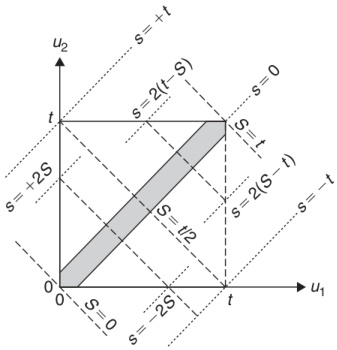
\includegraphics[width=0.30\textwidth]{images/chap15_m27cbe596090a0cf8d4130e8b80d6889e.jpg}
\caption{二重积分 \(I\) 的积分上限与下限，以 \(S\) 和 \(s\) 为变量表示。}
\label{fig:15_15.2}
\end{figure}

其中

\begin{equation}\tag{15.3.26}\label{eq:15.3.26}
C = \int _ { - \infty } ^{\infty} K ( s ) d s .
\end{equation}

?\autoref{eq:15.3.25}??\autoref{eq:15.3.16}?????

\begin{equation}\tag{15.3.27}\label{eq:15.3.27}
\langle v ^{2} ( t ) \rangle = v ^{2} ( 0 ) e ^{- 2 t / \tau} + C \frac { \tau } { 2 } ( 1 - e ^{- 2 t / \tau} ) .
\end{equation}

当 \(t \to \infty\) 时，\(\langle v^2(t) \rangle\) 必须趋近于等分分布值 \(3kT/M\)；因此，

\begin{equation}\tag{15.3.28}\label{eq:15.3.28}
C = 6 k T / M \tau
\end{equation}

因此

\begin{equation}\tag{15.3.29}\label{eq:15.3.29}
\langle v ^{2} ( t ) \rangle = v ^{2} ( 0 ) + \left\{ \frac { 3 k T } { M } - v ^{2} ( 0 ) \right\} ( 1 - e ^{- 2 t / \tau} ) .
\end{equation}

我们注意到，如果 \(\nu^{2}(0)\) 本身等于等分分布值 \(3kT/M\)，那么 \(\langle\nu^{2}(t)\rangle\) 将始终保持不变，这表明一旦达到统计平衡，该系统便具有自然地持续存在的倾向。

?\autoref{eq:15.3.29}??\autoref{eq:15.3.6}?????????????????????? \(\langle r^{2}\rangle\) ? \(t\) ????????????

\begin{equation}\tag{15.3.30}\label{eq:15.3.30}
\frac { d ^{2} } { d t ^{2} } \langle r ^{2} \rangle + \frac { 1 } { \tau } \frac { d } { d t } \langle r ^{2} \rangle = 2 v ^{2} ( 0 ) e ^{- 2 t / \tau} + \frac { 6 k T } { M } ( 1 - e ^{- 2 t / \tau} ) ,
\end{equation}

其解为

\begin{equation}\tag{15.3.31}\label{eq:15.3.31}
\langle r ^{2} \rangle = v ^{2} ( 0 ) \tau ^{2} ( 1 - e ^{- t / \tau} ) ^{2} - \frac { 3 k T } { M } \tau ^{2} ( 1 - e ^{- t / \tau} ) ( 3 - e ^{- t / \tau} ) + \frac { 6 k T \tau } { M } t .
\end{equation}

解 (31) 满足初始条件------在 \(t=0\) 时，\(\langle r^{2}\rangle\) 和其一阶导数均变为零；此外，若取 \(v^{2}(0)=3kT/M\)，则该解可归结为先前所求得的解 (7)。再次强调，在 \(t\ll\tau\) 时，运动呈现可逆性，\(\langle r^{2}\rangle\) 约似 \(v^{2}(0)t^{2}\)；而在 \(t\gg\tau\) 时，则呈现不可逆性，\(\langle r^{2}\rangle\) 约似 \((6BkT)t\)。

? 15.3 ?? 15.4 ????????????? \(\langle v^{2}(t)\rangle\) ? \(\langle r^{2}(t)\rangle\) ????????????\autoref{eq:15.3.29}?\autoref{eq:15.3.31}?????????????????????????????

在布朗发现近 200 年、爱因斯坦和斯莫鲁霍夫斯基进行分析并由佩兰开展早期测量已逾 100 年之后，布朗运动依然是当代研究的热点话题。这一研究热潮的再度兴起，源于胶体在各个领域中技术重要性的不断提升，以及数字视频与计算机图像分析技术的蓬勃发展。一个有趣的例子是，韩等人（2006）在薄型显微镜载玻片上对椭球形颗粒的旋转运动和二维平移运动进行了细致的观测与分析。旋转布朗运动最早由爱因斯坦（1906b）进行分析，并由佩兰（1934、1936）首次实现测量。旋转模式和平移模式均遵循朗之万动力学进行扩散，但平移扩散与旋转扩散相互耦合------因为沿较长轴方向的平移扩散常数大于垂直方向的扩散常数。

\(^{11}\)可以验证的是，

\begin{equation}\tag{15.3.32}\label{eq:15.3.32}
\frac { d } { d t } \langle v ^{2} ( t ) \rangle = \frac { 2 } { \tau } \left[ v ^{2} ( \infty ) - \langle v ^{2} ( t ) \rangle \right] = - \frac { 2 } { \tau } \Delta \langle v ^{2} ( t ) \rangle ,
\end{equation}

其中 \(v^{2}(\infty)=3kT/M\)，而 \(\Delta\langle v^{2}(t)\rangle\) 则表示``相关量偏离其平衡值的偏差''。以这种形式的方程，我们得以获得``弛豫现象''的典型实例，其弛豫时间约为 \(\tau/2\)。

\begin{equation}
p _ { \theta } ( \Delta \theta , t ) = \frac { 1 } { \sqrt { 4 \pi D _ { \theta } t } } \exp \left( - \frac { ( \Delta \theta ) ^{2} } { 4 D _ { \theta } t } \right) ,
\end{equation}

\begin{equation}\tag{15.3.33}\label{eq:15.3.33}
p _ { \mathrm { a } } ( \Delta x _ { \mathrm { a } } , t ) = \frac { 1 } { \sqrt { 4 \pi D _ { \mathrm { a } } t } } \exp \left( - \frac { ( \Delta x _ { \mathrm { a } } ) ^{2} } { 4 D _ { \mathrm { a } } t } \right) ,
\end{equation}

\begin{equation}\tag{15.3.34}\label{eq:15.3.34}
p _ { \mathrm { b } } ( \Delta x _ { \mathrm { b } } , t ) = \frac { 1 } { \sqrt { 4 \pi D _ { \mathrm { b } } t } } \exp \left( - \frac { ( \Delta x _ { \mathrm { b } } ) ^{2} } { 4 D _ { \mathrm { b } } t } \right) ,
\end{equation}

其中扩散常数分别为 \(D_{\theta}\)、\(D_{\mathrm{a}}\) 和 \(D_{\mathrm{b}}\)。实验观测表明，在短时间尺度上（\(t\lesssim\tau_{\theta}=1/(2D_{\theta})\)），系统表现出复杂的二维空间扩散，这与朗之万理论的预测相符。而在长时期（\(t\gg\tau_{\theta}\)）的空间扩散则表现为各向同性，其扩散常数为 \(\overline{D}=(D_{\mathrm{a}}+D_{\mathrm{b}})/2\)。

\section{A ?????????}\label{a-ux8c10ux632fux5b50ux7684ux70edux5e03ux6717ux8fd0ux52a8}

与扩散热布朗粒子的分析方法类似，我们同样可以对处于谐振子势场中的粒子进行分析------该势场能够阻止粒子远离原点扩散，从而更全面地探究位置与速度响应函数之间的关系，以及波动功率谱之间的关联；参见卡普勒（1938年）和钱德拉塞卡尔（1943年）的相关研究。对于质量为 \(M\) 的热布朗粒子，在具有弹簧常数 \(M\omega_{0}^{2}\) 的谐振子势场中，其一维运动方程为

\begin{equation}\tag{15.3.35}\label{eq:15.3.35}
\frac { d ^{2} x } { d t ^{2} } + \gamma \frac { d x } { d t } + \omega _ { 0 } ^{2} x = \frac { F ( t ) } { M } ,
\end{equation}

其中 \(\gamma\)（即 \(6\pi\eta a/M\)）是流体中球形粒子的阻尼系数，该流体的粘度为 \(\eta\)。正如在扩散热布朗运动的情形下一样，作用力 \(F(t)\) 可以是随时间变化的外力，用于探索响应函数；也可以是由于与流体中分子碰撞而产生的随时间变化的随机力，用以分析系统的平衡波动。假设系统在遥远的过去处于平衡状态，则在时刻 \(t\) 的位置可由以下公式给出：

\begin{equation}\tag{15.3.36}\label{eq:15.3.36}
x ( t ) = \int _ { - \infty } ^{t} \chi _ { x x } ( t - t ^{\prime} ) F ( t ^{\prime} ) d t ^{\prime} ,
\end{equation}

其中

\begin{equation}\tag{15.3.37}\label{eq:15.3.37}
\chi _ { x x } ( s ) = \frac { 1 } { M \omega _ { 1 } } e ^{- \frac { \gamma s} { 2 } } \sin { ( \omega _ { 1 } s ) }
\end{equation}

是 \(xx\) 响应函数，\(\omega_{1}=\sqrt{\omega_{0}^{2}-\frac{\gamma^{2}}{4}}\)。12 速度响应则由以下公式给出：

\begin{equation}\tag{15.3.38}\label{eq:15.3.38}
\nu ( t ) = \int _ { - \infty } ^{t} \chi \nu x ( t - t ^{\prime} ) F ( t ^{\prime} ) d t ^{\prime} ,
\end{equation}

¹² 这种形式的响应函数假定振子处于欠阻尼状态。符号 \(\chi_{xx}\) 指的是第15.6.A节中所采用的符号，其中位置坐标 \(x\) 的响应依赖于施加的外场 \(F\)，而该外场通过一项项 \(-F(t)x(t)\) 与哈密顿量耦合。

其中

\begin{equation}\tag{15.3.39}\label{eq:15.3.39}
\chi _ { v x } ( s ) = \frac { 1 } { M } e ^{- \frac { \gamma s} { 2 } } \left( \cos ( \omega _ { 1 } s ) - \frac { \gamma } { 2 \omega _ { 1 } } \sin ( \omega _ { 1 } s ) \right) .
\end{equation}

系统的响应可以分解为一系列独立项的和，这些项涉及一个正弦形外加力 \(\hat{F}(\omega)e^{i\omega t}\)。其形式如下：

\begin{equation}\tag{15.3.40}\label{eq:15.3.40}
\hat { \chi } ( \omega ) = \tilde { \chi } _ { x x } ( \omega ) \hat { F } ( \omega ) ,
\end{equation}

其中，频率依赖的响应函数可以分解为实部和虚部 \(\hat{\chi}_{xx}^{\prime}(\omega)\) 和 \(\hat{\chi}_{xx}^{\prime\prime}(\omega)\)：

\begin{equation}\tag{15.3.41}\label{eq:15.3.41}
\tilde { \chi } _ { x x } ( \omega ) = \int _ { 0 } ^{\infty} \chi _ { x x } ( s ) e ^{i \omega s} d s = \hat { \chi } _ { x x } ^{\prime} ( \omega ) + i \hat { \chi } _ { x x } ^{\prime \prime} ( \omega ) ,
\end{equation}

\begin{equation}\tag{15.3.42}\label{eq:15.3.42}
\hat { \chi } _ { x x } ^{\prime} ( \omega ) = \frac { \omega _ { 0 } ^{2} - \omega ^{2} } { M [ ( \omega _ { 0 } ^{2} - \omega ^{2} ) ^{2} + \gamma ^{2} \omega ^{2} ] } ,
\end{equation}

\begin{equation}\tag{15.3.43}\label{eq:15.3.43}
\hat { \chi } _ { x x } ^{\prime \prime} ( \omega ) = \frac { \gamma \omega } { M [ ( \omega _ { 0 } ^{2} - \omega ^{2} ) ^{2} + \gamma ^{2} \omega ^{2} ] } .
\end{equation}

这里的实部描述了色散特性，而虚部则描述了耗散特性，即它决定了由于正弦形外力而产生的能量平均耗散速率。

现在，我们来考虑粒子在平衡状态下的位置与速度的自然涨落，这些涨落是由于与流体中原子的随机碰撞所引起的。我们将沿用先前用于自由粒子布朗运动的相同朗之万框架。随机力的平均值为零，并且假设其在时间上呈δ函数相关性：

\begin{equation}\tag{15.3.44}\label{eq:15.3.44}
\begin{array}{rlr} & { } & { \langle F \rangle = 0 , } \\& { } & { \langle F ( t ) F ( t ^{\prime} ) \rangle = \Gamma \delta ( t - t ^{\prime} ) , } \end{array}
\end{equation}

其中，\(\Gamma = 2\gamma MkT\)。按照这一选择，粒子的长期平均位置和速度均为零，

\begin{equation}\tag{15.3.45}\label{eq:15.3.45}
\langle x ( t ) \rangle = \langle v ( t ) \rangle = 0 ,
\end{equation}

而且，位置与速度平方的平均值均遵循等能分布定理：

\begin{equation}\tag{15.3.46}\label{eq:15.3.46}
\langle x ^{2} ( t ) \rangle = \frac { k T } { M \omega _ { 0 } ^{2} } ,  \langle v ^{2} ( t ) \rangle = \frac { k T } { M } .
\end{equation}

\(xx\)相关函数由以下公式给出：

\begin{equation}\tag{15.3.47}\label{eq:15.3.47}
\begin{array}{rl} & { G _ { x x } ( t - t ^{\prime} ) = \left\langle x ( t ) x ( t ^{\prime} ) \right\rangle } \\& {  = \frac { k T } { M \omega _ { 0 } ^{2} } \exp \left( \frac { - \gamma | t - t ^{\prime} | } { 2 } \right) \left( \cos \left( \omega _ { 1 } | t - t ^{\prime} | \right) + \frac { \gamma } { 2 \omega _ { 1 } } \sin \left( \omega _ { 1 } | t - t ^{\prime} | \right) \right) , } \end{array}
\end{equation}

而\(xx\)功率谱则由以下公式给出：

\begin{equation}\tag{15.3.48}\label{eq:15.3.48}
S _ { x x } ( \omega ) = \int _ { - \infty } ^{\infty} G _ { x x } ( s ) e ^{i \omega s} d s = \frac { 2 \gamma k T } { M } \frac { 1 } { \left( \omega _ { 0 } ^{2} - \omega ^{2} \right) ^{2} + \gamma ^{2} \omega ^{2} } .
\end{equation}

请注意，方程（39c）中响应函数的虚部 \(\hat{\chi}_{xx}''(\omega)\) 与功率谱 \(S_{xx}(\omega)\) 成正比：

\begin{equation}\tag{15.3.49}\label{eq:15.3.49}
\hat { \chi } _ { x x } ^{\prime \prime} ( \omega ) = \frac { \omega } { 2 k T } S _ { x x } ( \omega ) .
\end{equation}

这一结果表明，通过外力将系统从平衡态驱离所导致的耗散，与平衡状态下自然涨落的功率谱成正比。尽管这一结果最初是针对一种非常特定的模型推导出来的，但它却为我们将在第15.6节中推导出的通用波动-耗散定理提供了一个典型范例。

15.4 理论接近平衡：福克-普朗克方程

????????????????????????????????????? \(r(t)\) ??? \(v(t)\) ?????????????????????????????????????????????????????????????????????15.2???????????????????????????\autoref{eq:15.2.20}????????? \(n(r,t)\)????\autoref{eq:15.2.22}????????? \(\langle r^2(t) \rangle\)?

一种更为通用的视角，用来理解``给定布朗粒子分布如何以及以何种速率接近热力学平衡状态''，是通过所谓的``主方程''来实现的。主方程的简化版本被称为福克-普朗克方程。为作说明，我们考察一组粒子沿 \(x\) 轴的位移 \(x(t)\)。在任意时刻 \(t\)，设 \(f(x,t)dx\) 表示集合中任意一个粒子可能在 \(x\) 与 \(x+dx\) 之间发生位移的概率。该函数

\(f(x,t)\) 必须满足归一化条件

\begin{equation}\tag{15.4.1}\label{eq:15.4.1}
\int _ { - \infty } ^{\infty} f ( x , t ) d x = 1 .
\end{equation}

主方程可写成：

\begin{equation}\tag{15.4.2}\label{eq:15.4.2}
\frac { \partial f ( x , t ) } { \partial t } = \int _ { - \infty } ^{\infty} \{ - f ( x , t ) W ( x , x ^{\prime} ) + f ( x ^{\prime} , t ) W ( x ^{\prime} , x ) \} d x ^{\prime} ,
\end{equation}

其中 \(W(x,x')dx'\delta t\) 表示，在短时间间隔 \(\delta t\) 内，一个位移为 \(x\) 的粒子，转变为位移为 \(x'\) 的概率。13

方程（2）中的积分第一部分，对应于所有将粒子从时间 \(t\) 时的位移 \(x\) 转移到其他位移 \(x'\) 的转变过程，因此构成了函数 \(f(x,t)\) 的净损失；同样地，积分第二部分则对应于所有将粒子从时间 \(t\) 时的其他位移 \(x'\) 转移到位移 \(x\) 的转变过程，因而构成了函数 \(f(x,t)\) 的净收益。14

主方程的结构正是建立在极其简单且直白的前提之上的。当然，在特定条件下，该方程，或其任何推广形式（例如包含速度或动量等坐标参数的版本），都可以被简化为简单的形式

\begin{equation}\tag{15.4.3}\label{eq:15.4.3}
\frac { \partial f } { \partial t } = - \frac { f - f _ { 0 } } { \tau } ,
\end{equation}

这一形式已被证明是研究与传输现象相关问题时非常有用的首次近似方法。在此，\(f_0\) 表示平衡分布函数（当 \(f=f_0\) 时，\(\partial f/\partial t=0\)），而 \(\tau\) 则是弛豫时间，它决定了系统中波动的传播速率，从而决定系统最终达到平衡状态的速度。

在基于式（2）研究布朗运动时，我们可以放心地假设：只有在``紧密相邻''的状态 \(x\) 和 \(x'\) 之间发生的跃迁才具有可观的几率；换言之，跃迁概率函数 \(W(x, x')\) 在 \(x' = x\) 这一值附近呈现出尖峰状分布，并在 \(x\) 之外迅速趋近于零。将区间 \((x' - x)\) 记为 \(\xi\)，我们可写作

\begin{equation}\tag{15.4.4}\label{eq:15.4.4}
W ( x , x ^{\prime} ) \rightarrow W ( x ; \xi ) , \ W ( x ^{\prime} , x ) \rightarrow W ( x ^{\prime} ; - \xi )
\end{equation}

¹³ 我们在此暗中假定一种``马尔可夫''情形：跃迁概率函数 \(W(x, x')\) 仅取决于粒子当前的位置 \(x\)（当然也包括其后续位置 \(x'\)），而与粒子的先前历史无关。

¹⁴ 对于费米子而言，必须考虑泡利不相容原理，该原理决定了系统中``单粒子态的占据情况''；例如，在这种情况下，我们不能考虑那样一种跃迁：该跃迁会将一个粒子转移到一个已经处于占据状态的态。为此，我们需要对主方程进行适当的修正。

其中 \(W(x; \xi)\) 和 \(W(x'; -\xi)\) 在 \(\xi=0\) 这一值附近具有尖峰，并在其他地方迅速趋近于零。¹⁵ 这使我们能够将式（2）的右侧在 \(\xi=0\) 附近展开为泰勒级数。仅保留至二阶项，我们得到

\begin{equation}\tag{15.4.5}\label{eq:15.4.5}
\frac { \partial f ( x , t ) } { \partial t } = - \frac { \partial } { \partial x } \{ \mu _ { 1 } ( x ) f ( x , t ) \} + \frac { 1 } { 2 } \frac { \partial ^{2} } { \partial x ^{2} } \{ \mu _ { 2 } ( x ) f ( x , t ) \} ,
\end{equation}

其中

\begin{equation}\tag{15.4.6}\label{eq:15.4.6}
\mu _ { 1 } ( x ) = \int _ { - \infty } ^{\infty} \xi W ( x ; \xi ) d \xi = \frac { \langle \delta x \rangle _ { \delta t } } { \delta t } = \langle v _ { x } \rangle
\end{equation}

以及

\begin{equation}\tag{15.4.7}\label{eq:15.4.7}
\mu _ { 2 } ( x ) = \int _ { - \infty } ^{\infty} \xi ^{2} W ( x ; \xi ) d \xi = \frac { \langle ( \delta x ) ^{2} \rangle _ { \delta t } } { \delta t } .
\end{equation}

式（5）即所谓的福克-普朗克方程，它在布朗运动与涨落领域中占据着经典的地位。

??????????????????????????????????????? \(F_{x} = -\lambda x\) ????????????????? \(B\)????????????\autoref{eq:15.3.4}????? \(\tau\)?? \(MB\)???????????? \(t\) ???????? \(\tau\) ??????????????? \(-\langle v_{x}\rangle/B\) ???????????????

\begin{equation}\tag{15.4.8}\label{eq:15.4.8}
- \frac { \langle v _ { x } \rangle } { B } + F _ { x } = 0
\end{equation}

因此

\begin{equation}\tag{15.4.9}\label{eq:15.4.9}
\langle v _ { x } \rangle \equiv \mu _ { 1 } ( x ) = - \lambda B x .
\end{equation}

??????\autoref{eq:15.3.10}????

\begin{equation}\tag{15.4.10}\label{eq:15.4.10}
\frac { \langle ( \delta x ) ^{2} \rangle } { \delta t } \equiv \mu _ { 2 } ( x ) = 2 B k T ;
\end{equation}

值得注意的是，此处我们忽略了 \(\lambda\) 对这一量的影响。将式（9）和式（10）代入式（5），我们得到

\begin{equation}\tag{15.4.11}\label{eq:15.4.11}
\frac { \partial f } { \partial t } = \lambda B \frac { \partial } { \partial x } ( x f ) + B k T \frac { \partial ^{2} f } { \partial x ^{2} } .
\end{equation}

\(^{15}\)显然，这一假设将我们的分析范围限制在所谓的``布朗运动近似''范畴内------在这种情况下，我们假定所研究的对象与构成环境的分子之间存在着数量级上的巨大差异。显而易见，若试图用这种分析方法来``理解''分子自身的运动行为，那么我们所能期待的，无非是得出一种``粗略、半定量''的结果。

现在，我们将方程（11）应用于一组布朗粒子，这些粒子最初集中于点 \(x = x_0\)。首先，我们注意到，在没有恢复力的情况下（即 \(\lambda = 0\)），方程（11）会简化为一维扩散方程。

\begin{equation}\tag{15.4.12}\label{eq:15.4.12}
\frac { \partial f } { \partial t } = D \frac { \partial ^{2} f } { \partial x ^{2} }  ( D = B k T ) ,
\end{equation}

???????????\autoref{eq:15.2.19}?\autoref{eq:15.3.11}?????????????????????????????????\autoref{eq:15.2.20}?????? \(f(x,t)\) ????

\begin{equation}\tag{15.4.13}\label{eq:15.4.13}
f ( x , t ) = \frac { 1 } { ( 4 \pi D t ) ^{1 / 2} } \exp \left\{ - \frac { ( x - x _ { 0 } ) ^{2} } { 4 D t } \right\} ,
\end{equation}

其中

\begin{equation}\tag{15.4.14}\label{eq:15.4.14}
{ \overline { { x } } } = x _ { 0 }  { \mathrm { a n d } }  { \overline { { x ^{2} } } } = x _ { 0 } ^{2} + 2 D t ;
\end{equation}

最后的结果表明，粒子所行进的平均平方距离会随时间线性增长，且其值并无上限。然而，恢复力却对粒子的扩散趋势起到了制约作用。例如，在存在此类力（\(\lambda \neq 0\)）的情况下，终端分布 \(f_{\infty}\)（此时 \(\partial f/\partial t = 0\)）由下式决定：

\begin{equation}\tag{15.4.15}\label{eq:15.4.15}
\frac { \partial } { \partial x } ( x f _ { \infty } ) + \frac { k T } { \lambda } \frac { \partial ^{2} f _ { \infty } } { \partial x ^{2} } = 0 ,
\end{equation}

该方程给出

\begin{equation}\tag{15.4.16}\label{eq:15.4.16}
f _ { \infty } ( x ) = \left( \frac { \lambda } { 2 \pi k T } \right) ^{1 / 2} \exp \left( - \frac { \lambda x ^{2} } { 2 k T } \right) ,
\end{equation}

其中

\begin{equation}\tag{15.4.17}\label{eq:15.4.17}
{ \overline { { x } } } = 0  { \mathrm { a n d } }  { \overline { { x ^{2} } } } = k T / \lambda .
\end{equation}

最后的结果表明，粒子 \(x\) 的平均平方值最终必须符合能量均分定理，即 \((\frac{1}{2}\lambda x^2)_{\infty} = \frac{1}{2}kT\)。从平衡统计力学的角度来看，如果我们把具有动能 \(p_x^2/2m\) 和势能 \(\frac{1}{2}\lambda x^2\) 的布朗粒子视为与温度为 \(T\) 的热环境松散耦合，则我们可以直接写出：

\begin{equation}\tag{15.4.18}\label{eq:15.4.18}
f _ { e q } ( x , p _ { x } ) d x d p _ { x } \propto e ^{- ( p _ { x} ^{2} / 2 m + \lambda x ^{2} / 2 ) / k T } d x d p _ { x } .
\end{equation}

通过对 \(p_x\) 进行积分，表达式（18）可直接导出分布函数（16）。

\begin{equation}
p ( x , t ) = \left\{ \frac { \lambda } { 2 \pi k T ( 1 - e ^{- 2 \lambda B t} ) } \right\} ^{1 / 2} \exp \left\{ - \frac { \lambda ( x - x _ { 0 } e ^{- \lambda B t} ) ^{2} } { 2 k T ( 1 - e ^{- 2 \lambda B t} ) } \right\} ,
\end{equation}

其中

\begin{equation}\tag{15.4.19}\label{eq:15.4.19}
\overline { { x } } = x _ { 0 } e ^{- \lambda B t}  \mathrm { a n d }  \overline { { x ^{2} } } = x _ { 0 } ^{2} e ^{- 2 \lambda B t} + \frac { k T } { \lambda } ( 1 - e ^{- 2 \lambda B t} ) ;
\end{equation}

在极限情形下，当\(\lambda \to 0\)时，我们可恢复到纯粹的``扩散''状态，正如方程（13）和（14）所描述的那样；而当\(t \gg (\lambda B)^{-1}\)时，我们则会趋近于``终端''状态，如方程（16）和（17）所描述的那样。图15.5展示了在恢复力与分子碰撞的共同作用下，一整组布朗运动粒子如何逐渐接近平衡态；显然，当前过程的弛豫时间约为\((\lambda B)^{-1}\)。

上述理论易于应用于的一种物理系统，便是动圈式检流计的振荡部分。在此系统中，我们使用一根细丝将线圈与反射镜悬挂在空中，使它们能够绕垂直轴旋转。空气分子与悬吊系统之间的随机、无规则的碰撞会产生一系列强度不断变化的转矩；因此，系统的角位置\(\theta\)不断波动，系统呈现出一种非稳态的零值。这显然是布朗运动的又一个典型例子！在这种情况下，粘性力的作用由检流计的空气阻尼机制（或称电磁阻尼）来承担，而恢复转矩\(N_{\theta} = -c\theta\)则源于细丝的扭转特性。在平衡状态下，我们

预计

\begin{equation}\tag{15.4.20}\label{eq:15.4.20}
\overline { { \left( \frac { 1 } { 2 } c \theta ^{2} \right) } } = \frac { 1 } { 2 } k T ,  \mathrm { t h a t ~ i s , }  \overline { { \theta ^{2} } } = \frac { k T } { c } ;
\end{equation}

将此与方程（17）进行比较。卡普勒（1931）对这类系统的均方偏移量\(\theta^{2}\)进行了实验测定，并将他的研究成果用于推导出一个基于方程（21）的经验公式，从而得到了玻尔兹曼常数\(k\)（或者更确切地说，阿伏伽德罗常数\(N_{A}\)）的数值。卡普勒所使用的系统，其转动惯量\(I=4.552\times10^{-4}\,\mathrm{g}\,\mathrm{cm}^{2}\)，振荡周期\(\tau=1379\,\mathrm{s}\)；据此，恢复转矩的常数\(c\)的值可通过公式\(\tau=2\pi(I/c)^{1/2}\)计算得出，因此

\begin{equation}\tag{15.4.21}\label{eq:15.4.21}
c = 4 \pi ^{2} ( I / \tau ^{2} ) = 9 . 44 3 \times 10 ^{- 9} \mathrm { g } \, \mathrm { c m } ^{2} \mathrm { s } ^{- 2} / \mathrm { r a d } .
\end{equation}

在287.1 K的温度下，观测到的\(\overline{\theta^{2}}\)值为\(4.178 \times 10^{-6}\)。将这些数值代入方程（21），卡普勒得出了：\(k = 1.374 \times 10^{-16}\) erg K\(^{-1}\)。由于气体常数\(R\)等于\(8.31 \times 10^{7}\) erg K\(^{-1}\) mol\(^{-1}\)，他由此推导出阿伏伽德罗常数：\(N_{A} = R/k = 6.06 \times 10^{23}\) mol\(^{-1}\)。

人们或许会认为，将镜像系统置于``真空''外壳中，可以大幅降低由空气分子碰撞所引起的波动。然而事实并非如此------即便在最低可能的压强下，系统中仍然存在着数量极其庞大的分子，它们持续``维持''着布朗运动的活跃状态。不过，故事中颇为有趣的一点在于：由于分子轰击而引起的系统均方偏移量，并不会受到分子密度的影响；对于处于平衡状态的系统而言，这一值完全由温度决定。这一情形在图15.6中得到了极为生动的呈现：图中我们分别绘制了镜像系统的两次振荡曲线，上部曲线是在大气压下获得的，而下部曲线则是在10⁻⁴毫米汞柱的压力下采集的。在这两种情况下，均方根偏差几乎完全相同！尽管如此，我们仍能察觉到这两条曲线之间存在``质量''上的差异，这种差异与波动的``频谱''有关，并且其成因如下：当周围气体的密度较高时，分子脉冲会迅速接连不断，导致系统各次偏移的数量众多，但幅度却相对较小；随着气压的降低， successive脉冲之间的时长逐渐延长，使得每次偏移的数量减少，但幅度却有所增加。然而，无论在长时间内观测到的整体偏移量，其数值基本保持不变。

\begin{figure}[htbp]
\centering
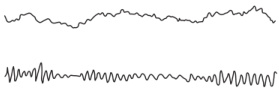
\includegraphics[width=0.25\textwidth]{images/chap15_m157329fad266fd2d2fa6dc87e549cb00.jpg}
\caption{两幅悬挂在空气中的镜像系统热振动曲线；上部曲线为大气压，下部曲线为 \(10^{-4}\) mmHg。}
\label{fig:15_15.6}
\end{figure}

其中

\begin{equation}\tag{15.4.22}\label{eq:15.4.22}
a _ { 0 } = \frac { 1 } { T } \int _ { 0 } ^{T} y ( t ) d t ,
\end{equation}

\begin{equation}\tag{15.4.23}\label{eq:15.4.23}
a _ { n } = \frac { 2 } { T } \int _ { 0 } ^{T} y ( t ) \cos ( 2 \pi n f _ { 0 } t ) d t ,
\end{equation}

以及

\begin{equation}\tag{15.4.24}\label{eq:15.4.24}
b _ { n } = \frac { 2 } { T } \int _ { 0 } ^{T} y ( t ) \sin ( 2 \pi \, n f _ { 0 } t ) d t ;
\end{equation}

在这种情况下，系数 \(a\) 和 \(b\) 将完全确定，并且能够毫无误差地定义变量 \(y(t)\) 的频谱。反之，如果给定的

变量在某种程度上更像是随时间随机变化的函数，那么系数 \(a\) 和 \(b\) 自身就具有统计学性质。要将周期性这一概念应用于此类函数，我们必须将``重复的时间间隔''取为无穷大，即让 \(f_0 \to 0\)。

???????????\autoref{eq:15.4.3}????

\begin{equation}\tag{15.4.25}\label{eq:15.4.25}
a _ { 0 } = \operatorname* { L i m } _ { T \to \infty } { \frac { 1 } { T } } \int _ { 0 } ^{T} y ( t ) d t \equiv \langle y ( t ) \rangle ;
\end{equation}

因此，表示变量 \(y\) 平均值（或直流值）的系数 \(a_{0}\)，既可以通过对该变量进行时间平均（在足够长的时间区间内）来确定，也可以通过在任意时刻 \(t\) 进行集合平均来确定。为了方便起见，且不损失一般性，我们取 \(a_{0}=0\)；换句话说，我们假设已从变量 \(y(t)\) 的实际数值中减去了其平均值 \(\langle y(t)\rangle\)。16

???\autoref{eq:15.4.4}?\autoref{eq:15.4.5}??????????????? \(n\)?

\begin{equation}\tag{15.4.26}\label{eq:15.4.26}
\langle a _ { n } \rangle = \langle b _ { n } \rangle = 0 .
\end{equation}

??????\autoref{eq:15.4.2}??????????????

\begin{equation}\tag{15.4.27}\label{eq:15.4.27}
\begin{array}{rl} & { \langle y ^{2} ( t ) \rangle = \sum _ { n } \frac { 1 } { 2 } \langle a _ { n } ^{2} \rangle + \sum _ { n } \frac { 1 } { 2 } \langle b _ { n } ^{2} \rangle } \\& {  = \sum _ { n } \frac { 1 } { 2 } \Big \{ \langle a _ { n } ^{2} \rangle + \langle b _ { n } ^{2} \rangle \Big \} = \mathrm { c o n s t . } } \end{array}
\end{equation}

? \(\frac{1}{2}\{\langle a_{n}^{2}\rangle+\langle b_{n}^{2}\rangle\}\) ????? \(nf_{0}\) ???????????? \(\langle y^{2}(t)\rangle\) ????????????????????????? \(n\)???? \(\langle a_{n}^{2}\rangle=\langle b_{n}^{2}\rangle\)????\autoref{eq:15.4.8}????

\begin{equation}\tag{15.4.28}\label{eq:15.4.28}
\langle y ^{2} \rangle = \sum _ { n } \langle a _ { n } ^{2} \rangle \simeq \int _ { 0 } ^{\infty} w ( f ) d f ,
\end{equation}

其中

\begin{equation}\tag{15.4.29}\label{eq:15.4.29}
\langle a _ { n } ^{2} \rangle = w ( n f _ { 0 } ) \, \Delta ( n f _ { 0 } ) ,  \mathrm { t h a t ~ i s , }  w ( n f _ { 0 } ) = \frac { 1 } { f _ { 0 } } \, \langle a _ { n } ^{2} \rangle ;
\end{equation}

函数 \(w(f)\) 定义了变量 \(y(t)\) 的功率谱。

现在我们来证明，随机变量 \(y(t)\) 的功率谱 \(w(f)\) 完全由其自相关函数 \(K(s)\) 确定。为此，我们借助于

方程（4），该方程给出了

\begin{equation}\tag{15.4.30}\label{eq:15.4.30}
\langle a _ { n } ^{2} \rangle = 4 f _ { 0 } ^{2} \int _ { 0 } ^{1 / f _ { 0} } \int _ { 0 } ^{1 / f _ { 0} } \langle y ( t _ { 1 } ) y ( t _ { 2 } ) \rangle \cos ( 2 \pi n f _ { 0 } t _ { 1 } ) \cos ( 2 \pi n f _ { 0 } t _ { 2 } ) d t _ { 1 } d t _ { 2 } .
\end{equation}

将变量替换为

\begin{equation}\tag{15.4.31}\label{eq:15.4.31}
S = \frac { 1 } { 2 } ( t _ { 1 } + t _ { 2 } )  \mathrm { a n d }  s = ( t _ { 2 } - t _ { 1 } ) ,
\end{equation}

并牢记，积分所作用的区间 \(T\) 比该随机变量``记忆''持续的时间要长得多，因此我们得到

\begin{equation}\tag{15.4.32}\label{eq:15.4.32}
\langle a _ { n } ^{2} \rangle \simeq 2 f _ { 0 } ^{2} \int _ { S = 0 } ^{1 / f _ { 0} } \int _ { s = - \infty } ^{\infty} K ( s ) \{ \cos ( 2 \pi n f _ { 0 } s ) + \cos ( 4 \pi n f _ { 0 } S ) \} d S d s ;
\end{equation}

将此与从方程（15.3.22）到（15.3.25）及（15.3.26）的推导步骤进行比较。在（12）中，积分中的第二部分在 S 上被积化为零；而第一部分则给出

\begin{equation}\tag{15.4.33}\label{eq:15.4.33}
\langle a _ { n } ^{2} \rangle = 4 f _ { 0 } \int _ { 0 } ^{\infty} K ( s ) \cos ( 2 \pi n f _ { 0 } s ) d s .
\end{equation}

将（13）与（10）进行对比，我们得到了所需的公式

\begin{equation}\tag{15.4.34}\label{eq:15.4.34}
w ( f ) = 4 \int _ { 0 } ^{\infty} K ( s ) \cos ( 2 \pi f s ) d s .
\end{equation}

对 \((14)\) 取逆运算，我们得到

\begin{equation}\tag{15.4.35}\label{eq:15.4.35}
K ( s ) = \int _ { 0 } ^{\infty} w ( f ) \cos ( 2 \pi f s ) d f .
\end{equation}

对于 \(s=0\)，公式（15）给出了一个重要的关系式

\begin{equation}\tag{15.4.36}\label{eq:15.4.36}
K ( 0 ) = \int _ { 0 } ^{\infty} w ( f ) d f = \langle y ^{2} \rangle ;
\end{equation}

同样请参阅方程（9），以及随机变量 \(y\) 自相关函数的定义------即 \(K(s) = \langle y(t_1)y(t_1 + s) \rangle\)。方程（14）和（15），它们连接了互补函数 \(w(f)\) 和 \(K(s)\)，构成了一个由维纳（1930年）和辛钦（1934年）命名的定理。

接下来，我们将探讨随机变量 \(y(t)\) 的一些特殊情况，以说明维纳-辛钦定理的应用。

情形一

如果给定的随机变量 \(y(t)\) 极其不规则、因而难以预测，那么其相关函数 \(K(s)\) 在时间区间 \(s\) 内的延伸范围将微乎其微。\(^{17}\) 我们可以这样写：

\begin{equation}\tag{15.4.37}\label{eq:15.4.37}
K ( s ) = c \delta ( s ) .
\end{equation}

方程（14）随后给出

\begin{equation}\tag{15.4.38}\label{eq:15.4.38}
w ( f ) = 2 c  { \mathrm { f o r ~ a l l ~ } } f .
\end{equation}

一种频谱，其在不同频率上的能量分布均匀，被称为``平坦''或``白色''频谱。然而，我们注意到，如果这种均匀分布在所有频率上------从 0 到 \(\infty\)------都真正成立，那么方程（16）中的积分，其值与 \(\langle y^2 \rangle\) 相同，却会发散！因此，我们预期，在任何现实情境中，相关函数 \(K(s)\) 都不会像（17a）那样尖峰陡峭。通常，\(K(s)\) 会在变量 \(s\) 的一个较小范围内延伸，大约为 \(O(\sigma)\)，而这一范围又会界定一个``频率带''，其频率 \(f = O(1/\sigma)\)，使得函数 \(w(f)\) 随着 \(f\) 跨越这一区域而发生性质变化：在较低频率时，\(w(f) \to \text{常数} \neq 0\)；而在较高频率时，\(w(f) \to \text{常数} = 0\)。图 15.7 展示了这种情形的一种可能表现形式，其中我们相当随意地

\begin{equation}\tag{15.4.39}\label{eq:15.4.39}
K ( s ) = K ( 0 ) \frac { \sin ( a s ) } { a s } \ \ ( a > 0 ) ,
\end{equation}

对于哪一种情况

\begin{equation}\tag{15.4.40}\label{eq:15.4.40}
\begin{array}{r} { w ( f ) = \frac { 2 \pi } { a } K ( 0 )  \mathrm { f o r }  f < \frac { a } { 2 \pi } } \\{ 0   \mathrm { f o r }  f > \frac { a } { 2 \pi } . } \end{array}
\end{equation}

??? \(a \to \infty\) ?????\autoref{eq:15.4.18}????\autoref{eq:15.4.17}??? \(c = \pi a^{-1}K(0)\)?

情形 2

另一方面，如果变量 \(y(t)\) 极其规则，因而具有可预测性，那么其相关函数会在较大的 \(s\) 值范围内延伸；其功率谱则会以``峰值''的形式呈现，这些峰值位于该变量的若干``特征频率''处。在最简单的单色变量情形下，若其特征频率为 \(f^{*}\)，相关函数将为：

\begin{equation}\tag{15.4.41}\label{eq:15.4.41}
K ( s ) = K ( 0 ) \cos ( 2 \pi f ^{*} s ) ,
\end{equation}

¹⁷ 这一结论在很大程度上适用于布朗粒子因不断接收到的分子脉冲而所经历的快速波动力 \(F(t)\)。

\begin{figure}[htbp]
\centering
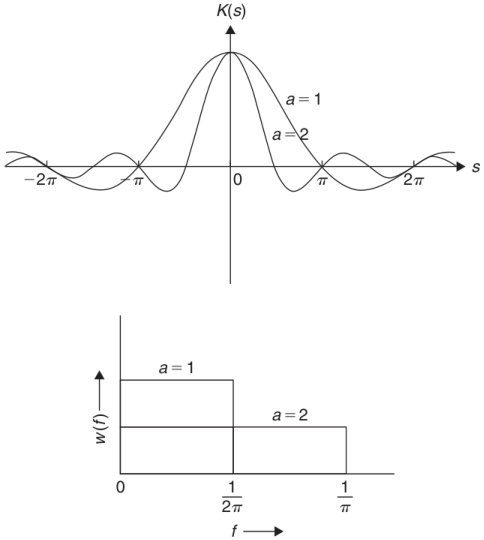
\includegraphics[width=0.43\textwidth]{images/chap15_m4c8e55bacef9097ae461169479aa19e6.jpg}
\caption{给定变量 \(y(t)\) 的自相关函数 \(K(s)\) 与功率分布函数 \(w(f)\)。}
\label{fig:15_15.7}
\end{figure}

这确实满足以下关系

\begin{equation}\tag{15.4.42}\label{eq:15.4.42}
\begin{array}{r} { \int _ { 0 } ^{\infty} w ( f ) d f = \frac { 2 k T } { \pi M } \tan ^{- 1} ( 2 \pi f \tau ) \Big | _ { 0 } ^{\infty} } \\{ = \frac { k T } { M } = \langle v _ { x } ^{2} \rangle , } \end{array}
\end{equation}

与单个速度分量 \(\boldsymbol{\nu}\) 所适用的等能分配定理相一致。对于 \(f \ll \tau^{-1}\)，功率分布几乎与 \(f\) 无关，这意味着功率谱近乎``白噪声''状，且具有

\begin{equation}\tag{15.4.43}\label{eq:15.4.43}
w ( f ) \simeq \frac { 4 k T \tau } { M } = 4 B k T .
\end{equation}

\begin{figure}[htbp]
\centering
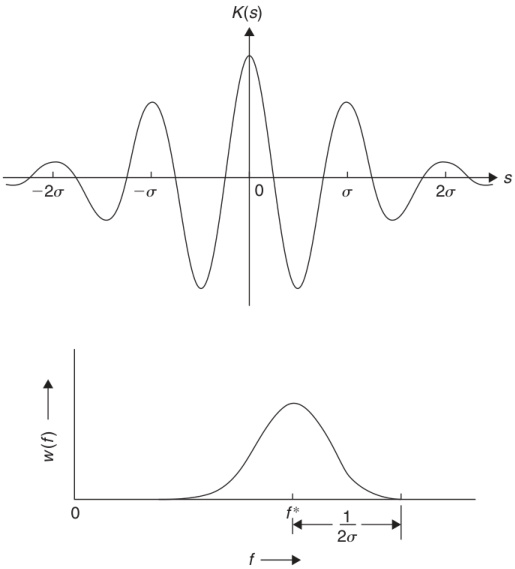
\includegraphics[width=0.46\textwidth]{images/chap15_m218f5b9f42080ef0f3008340a988b90c.jpg}
\caption{窄带滤波变量的自相关函数与功率分布函数示意。}
\label{fig:15_15.9}
\end{figure}
于是我们可以将频率区间 \((f, f+\Delta f)\) 内的速度波动进行如下表示，其中 \(f \ll \tau^{-1}\)，

\begin{equation}\tag{15.4.44}\label{eq:15.4.44}
\langle \Delta v _ { x } ^{2} \rangle _ { ( f , f + \Delta f ) } \simeq w ( f ) \Delta f \simeq ( 4 B k T ) \Delta f .
\end{equation}

一般来说，我们的测量仪器（或者在对粒子进行视觉检查时，用眼睛）都具有有限的响应时间 \(\tau_{0}\)，因此它无法对高于 \(\tau_{0}^{-1}\) 的频率作出响应。此时，观测到的波动可以用``修剪''后的表达式来描述：

\begin{equation}\tag{15.4.45}\label{eq:15.4.45}
\langle v _ { x } ^{2} \rangle _ { \mathrm { o b s } } \simeq \int _ { 0 } ^{1 / \tau _ { 0} } w ( f ) d f = \frac { 2 k T } { \pi M } \tan ^{- 1} \left( 2 \pi \frac { \tau } { \tau _ { 0 } } \right) ,
\end{equation}

而不是使用``完整''的表达式（22）。在典型情况下，布朗粒子的质量 \(M \sim 10^{-12}\) 克，其直径 \(2a \sim 10^{-4}\) 厘米，流体的粘度系数 \(\eta \sim 10^{-2}\) 派斯，因此弛豫时间 \(\tau = M/(6\pi\eta a) \sim 10^{-7}\) 秒。然而，在进行视觉观察时，响应时间 \(\tau_0\) 大约是 \(10^{-1}\) 秒；显然，\(\tau/\tau_0 \sim 10^{-6} \ll 1\)。

方程（25）随后简化为\(^{18}\)

\begin{equation}\tag{15.4.46}\label{eq:15.4.46}
\langle v _ { x } ^{2} \rangle _ { \mathrm { o b s } } \simeq \frac { 4 k T \tau } { M \tau _ { 0 } } \ll \frac { k T } { M } ;
\end{equation}

因此，鉴于响应时间 \(\tau_{0}\) 是有限的，布朗粒子的观测均方根速度将被降低至 \(2(\tau/\tau_{0})^{1/2} \sim 10^{-3}\)；从数值上看，这使得均方根速度从室温下的 \(\sim 10^{-1}\) 厘米/秒降至 \(\sim 10^{-4}\) 厘米/秒。

令人欣慰的是，实际对布朗粒子的观测结果与这一结论完全一致；有关此问题的更详细分析，请参阅麦克唐纳（1950）。上述讨论凸显出这样一个事实：在对波动变量进行观测的过程中，我们的测量仪器只能捕捉到有限范围内的频率信号（由仪器的响应时间决定）；而更高频率的信号则会被直接忽略。

本节的理论可轻松应用于 \((L,R)\) 电路中电子运动的波动。对应于方程（21）至（24），我们现在可以针对电流 \(I\) 的波动得出：

\begin{equation}\tag{15.4.47}\label{eq:15.4.47}
w ( f ) = \frac { 4 k T \tau ^{\prime} } { L } \frac { 1 } { 1 + ( 2 \pi f \tau ^{\prime} ) ^{2} }  \left( \tau ^{\prime} = \frac { L } { R } \right) ,
\end{equation}

由此，

\begin{equation}\tag{15.4.48}\label{eq:15.4.48}
\int _ { 0 } ^{\infty} w ( f ) d f = \frac { k T } { L } = \langle I ^{2} \rangle ,
\end{equation}

与能量均分定理相符：\(\langle\frac{1}{2}LI^{2}\rangle=\frac{1}{2}kT\)。对于 \(f \ll 1/\tau'\)，方程（27）可简化为

\begin{equation}\tag{15.4.49}\label{eq:15.4.49}
w ( f ) \simeq \frac { 4 k T } { R } ,
\end{equation}

这再次表明存在``白噪声''；相应地，对于低频，

\begin{equation}\tag{15.4.50}\label{eq:15.4.50}
\langle \Delta I ^{2} \rangle _ { ( f , f + \Delta f ) } \simeq w ( f ) \Delta f \simeq \frac { 4 k T } { R } \Delta f .
\end{equation}

等价地，我们得到电压波动的表达式为

\begin{equation}\tag{15.4.51}\label{eq:15.4.51}
\langle \Delta V ^{2} \rangle _ { ( f , f + \Delta f ) } \simeq ( 4 R k T ) \Delta f .
\end{equation}

方程（31）构成了所谓的奈奎斯特定理。该定理最早由约翰逊（1927a、b；1928）通过经验发现，后来由奈奎斯特（1927--1928）基于以下原理加以推导：

这一结论涉及热力学第二定律，以及在热平衡状态下，两个电阻之间能量交换的有关论述。\(^{19}\)

\section{波动-耗散定理}\label{ux6ce2ux52a8-ux8017ux6563ux5b9aux7406}

在第15.3节中，我们得到了一项极为重要的结果，即

\begin{equation}\tag{15.4.52}\label{eq:15.4.52}
\begin{array}{rl} & { \frac { 1 } { B } \equiv \frac { M } { \tau } = \frac { M ^{2} } { 6 k T } C = \frac { M ^{2} } { 6 k T } \int _ { - \infty } ^{\infty} K _ { A } ( s ) d s } \\& { = \frac { 1 } { 6 k T } \int _ { - \infty } ^{\infty} K _ { F } ( s ) d s ; } \end{array}
\end{equation}

??\autoref{eq:15.3.4}?\autoref{eq:15.3.26}?\autoref{eq:15.3.28}????\(K_{A}(s)\) ? \(K_{F}(s)\) ???????????????? \(A(t)\) ???? \(F(t)\) ???????

\begin{equation}\tag{15.4.53}\label{eq:15.4.53}
K _ { A } ( s ) = \langle A ( 0 ) \cdot A ( s ) \rangle = \frac { 1 } { M ^{2} } \langle F ( 0 ) \cdot F ( s ) \rangle = \frac { 1 } { M ^{2} } K _ { F } ( s ) .
\end{equation}

???1???????????????????????????????? \(\mathcal{F}(t)\) ??????????? \(1/B\)??????????? \(F(t)\) ??????????????????????\autoref{eq:15.3.2}????????????????????????????????????????????????????1?????????????-?????

该定理最引人注目的特征在于：它以一种根本性的方式，将某一给定系统处于平衡状态时所对应的物理量的波动，与一种耗散过程联系起来------而这种耗散过程在实践中，只有当系统受到外力驱动、使其偏离平衡状态时才会真正发生。由此，我们得以借助对系统在处于某一平衡状态时所发生的热涨落的了解，来确定该系统的非平衡性质。

\(^{19}\)我们注意到，上述结果与爱因斯坦关于导体中电荷波动的原始结果本质上是等价的，即

\begin{equation}\tag{15.4.54}\label{eq:15.4.54}
\langle \delta q ^{2} \rangle _ { t } = \frac { 2 k T } { R } \, t ;
\end{equation}

同样值得注意的是，布朗粒子的结果为：\(\langle x^{2}\rangle_{t}=2BkTt\)。

\(^{20}\)???????? \(K_{A}(s)\) ? \(K_{F}(s)\) ?? \(s=O(\tau^{*})\) ?????\autoref{eq:15.3.21}??????????????????????

\begin{equation}\tag{15.4.55}\label{eq:15.4.55}
K _ { A } ( s ) = \frac { 6 k T } { M ^{2} B } \delta \left( s \right)  \mathrm { a n d }  K _ { F } ( s ) = \frac { 6 k T } { B } \delta ( s ) .
\end{equation}

以这种形式，这些函数仅在 \(s=0\) 时非零。

本章内容！若需了解波动-耗散定理的详细讲解，读者可参考久保（1966）。

??????????????\autoref{eq:15.3.11}??????????? \(D\) ???? \(B\) ??????? \(D = BkT\)??????1?????????

\begin{equation}\tag{15.4.56}\label{eq:15.4.56}
\frac { 1 } { D } = \frac { 1 } { 6 ( k T ) ^{2} } \int _ { - \infty } ^{\infty} K _ { F } ( s ) d s .
\end{equation}

现在，扩散系数 \(D\) 可以直接与随机变量 \(v(t)\) 的自相关函数 \(K_{v}(s)\) 建立联系。为此，我们首先从这样一个事实出发：根据定义，

\begin{equation}\tag{15.4.57}\label{eq:15.4.57}
r ( t ) = \int _ { 0 } ^{t} v ( u ) d u ,
\end{equation}

由此可得

\begin{equation}\tag{15.4.58}\label{eq:15.4.58}
\langle r ^{2} ( t ) \rangle = \int _ { 0 } ^{t} \int _ { 0 } ^{t} \langle v ( u _ { 1 } ) \cdot v ( u _ { 2 } ) \rangle d u _ { 1 } d u _ { 2 } .
\end{equation}

???\autoref{eq:15.3.22}??????????????????

\begin{equation}\tag{15.4.59}\label{eq:15.4.59}
\langle r ^{2} ( t ) \rangle = \int _ { 0 } ^{t / 2} d S \int _ { - 2 S } ^{+ 2 S} K _ { v } ( s ) d s + \int _ { t / 2 } ^{t} d S \int _ { - 2 ( t - S ) } ^{+ 2 ( t - S )} K _ { v } ( s ) d s ;
\end{equation}

?????\autoref{eq:15.3.24}?????

????\autoref{eq:15.3.14}??? \(\nu(t)\)????????? \(\langle\nu^{2}(t)\rangle\) ?????????????? \(\nu(t)\) ?????? \(K_{\nu}(s)\)?? \(\langle\nu^{2}(t)\rangle\) ???????????? \(K_{\nu}(0)\)????????

\begin{equation}\tag{15.4.60}\label{eq:15.4.60}
K _ { \nu } ( s ) = \left\{ \begin{array}{ll} { \nu ^{2} ( 0 ) e ^{- ( 2 t + s ) / \tau} + \frac { 3 k T } { M } e ^{- s / \tau} \left( 1 - e ^{- 2 t / \tau} \right) } & {  \mathrm { f o r }  s > 0 } \\{ \nu ^{2} ( 0 ) e ^{- ( 2 t + s ) / \tau} + \frac { 3 k T } { M } e ^{s / \tau} \left( 1 - e ^{- 2 ( t + s ) / \tau} \right) } & {  \mathrm { f o r }  s < 0 ; } \end{array} \right.
\end{equation}

??????\autoref{eq:15.3.27}??????????????7?????8???????????????

\begin{equation}\tag{15.4.61}\label{eq:15.4.61}
K _ { v } ( s ) = v ^{2} ( 0 ) e ^{- | s | / \tau} + \left\{ \frac { 3 k T } { M } - v ^{2} ( 0 ) \right\} \left( e ^{- | s | / \tau} - e ^{- ( 2 t + s ) / \tau} \right)  \mathrm { f o r ~ a l l ~ } s ;
\end{equation}

?????\autoref{eq:15.3.29}?????????????????

\begin{equation}\tag{15.4.62}\label{eq:15.4.62}
K _ { \nu } ( s ) = \frac { 3 k T } { M } e ^{- | s | / \tau} ,
\end{equation}

这与性质（15.3.20）相一致。需要注意的是，自相关函数 \(K_{\nu}(s)\) 的时间尺度由布朗运动的弛豫时间 \(\tau\) 确定，而 \(\tau\) 的数值要远大于用于确定自相关函数 \(K_{A}(s)\) 和 \(K_{F}(s)\) 时间尺度的特征时间 \(\tau^{*}\)。

?????????????10?????6?????? \(\langle r^{2}\rangle\) ????15.3.7???????????9???????????15.3.31???????15.17????????

\begin{equation}\tag{15.4.63}\label{eq:15.4.63}
\langle r ^{2} \rangle \xrightarrow { t \gg \tau } 6 D t .
\end{equation}

在同样的极限条件下，式（6）会简化为

\begin{equation}\tag{15.4.64}\label{eq:15.4.64}
\langle r ^{2} \rangle \simeq \int _ { 0 } ^{t} d S \int _ { - \infty } ^{\infty} K _ { \nu } ( s ) d s = t \int _ { - \infty } ^{\infty} K _ { \nu } ( s ) d s .
\end{equation}

通过比较这两个结果，我们得到了所需的关联关系：

\begin{equation}\tag{15.4.65}\label{eq:15.4.65}
D = \frac { 1 } { 6 } \int _ { - \infty } ^{\infty} K _ { \nu } ( s ) d s .
\end{equation}

顺便指出，根据式（3）和式（13），我们有

\begin{equation}\tag{15.4.66}\label{eq:15.4.66}
\int _ { - \infty } ^{\infty} K _ { v } ( s ) d s \int _ { - \infty } ^{\infty} K _ { F } ( s ) d s = ( 6 k T ) ^{2} ;
\end{equation}

另请参见问题15.7。

对于那些涉及耗散机制的情形，用来描述涨落-耗散定理的方程得以灵活适应，这并不令人意外。例如，电子在电阻中的运动所引起的涨落，会催生出一种``自发''的热电动势，可记作 \(\mathcal{B}(t)\)。秉承朗之万理论的精神，这种电动势可以被分解为两部分：(i) 一个``平均化''后的部分，即 \(-RI(t)\)，它代表了该情形中的电阻（或耗散）成分；(ii) 一个``快速波动''的部分，即 \(V(t)\)，在较长的时间尺度上，其平均值会趋近于零。于是，电阻中的``自发''电流可由下式给出：

\begin{equation}\tag{15.4.67}\label{eq:15.4.67}
L \frac { d I } { d t } = - R I + V ( t ) ;  \langle V ( t ) \rangle = 0 .
\end{equation}

????????\autoref{eq:15.3.2}????????????????????? \(R\) ??? \(\mathbf{V}(t)\) ????????????????????1????13??????????

\begin{equation}\tag{15.4.68}\label{eq:15.4.68}
R = \frac { 1 } { 6 k T } \int _ { - \infty } ^{\infty} \langle V ( 0 ) \cdot V ( s ) \rangle d s
\end{equation}

或者，等价地，

\begin{equation}\tag{15.4.69}\label{eq:15.4.69}
\frac { 1 } { R } = \frac { 1 } { 6 k T } \int _ { - \infty } ^{\infty} \langle I ( 0 ) \cdot I ( s ) \rangle d s .
\end{equation}

Kubo 在 1957 年和 1959 年对上述结果进行了推广；例如，参见 Kubo（1965）中的问题 6.19，或 Wannier（1966）第 23.2 节。关于推广，电流密度 \(j(t)\) 可用如下表达式表示：

\begin{equation}\tag{15.4.70}\label{eq:15.4.70}
j _ { i } ( t ) = \sum _ { l } \int _ { - \infty } ^{t} E _ { l } ( t ^{\prime} ) \Phi _ { l i } ( t - t ^{\prime} ) d t ^{\prime}  ( i , l = x , y , z ) ;
\end{equation}

在此，\(E(t)\) 表示施加的电场，而

\begin{equation}\tag{15.4.71}\label{eq:15.4.71}
\Phi _ { l i } ( s ) = \frac { 1 } { k T } \langle j _ { l } ( 0 ) j _ { i } ( s ) \rangle .
\end{equation}

显然，量 \(kT\Phi_{li}(s)\) 是涨落向量 \(\mathbf{j}(t)\) 自相关张量的各分量。特别是，若我们考虑静态情形 \(E=(E,0,0)\)，则可得系统的电导率为

\begin{equation}\tag{15.4.72}\label{eq:15.4.72}
\begin{array}{r} { \sigma _ { x x } \equiv \frac { j _ { x } } { E } = \int _ { - \infty } ^{t} \Phi _ { x x } ( t - t ^{\prime} ) d t ^{\prime} = \int _ { 0 } ^{\infty} \Phi _ { x x } ( s ) d s } \\{ = \frac { 1 } { 2 k T } \int _ { - \infty } ^{\infty} \langle j _ { x } ( 0 ) j _ { x } ( s ) \rangle d s , } \end{array}
\end{equation}

这一结果可与式（17）相比较。另一方面，若我们取 \(E=(E\cos\omega t,0,0)\)，则得到

\begin{equation}\tag{15.4.73}\label{eq:15.4.73}
\sigma _ { x x } ( \omega ) = \frac { 1 } { 2 k T } \int _ { - \infty } ^{\infty} \langle j _ { x } ( 0 ) j _ { x } ( s ) \rangle e ^{- i \omega s} d s .
\end{equation}

对式（21）取逆矩阵，可得

\begin{equation}\tag{15.4.74}\label{eq:15.4.74}
\langle j _ { x } ( 0 ) j _ { x } ( s ) \rangle = \frac { k T } { \pi } \int _ { - \infty } ^{\infty} \sigma _ { x x } ( \omega ) e ^{i \omega s} d \omega .
\end{equation}

若我们现在假设 \(\sigma_{xx}(\omega)\) 不依赖于 \(\omega\)（因此，可简称为 \(\sigma\)），则

\begin{equation}\tag{15.4.75}\label{eq:15.4.75}
\langle j _ { x } ( 0 ) j _ { x } ( s ) \rangle = ( 2 k T \sigma ) \delta ( s ) ;
\end{equation}

???? 20?????15.5.17???????????????????????????????????

15.6.A ???????????-????

在本节中，我们将证明：热力学系统对微小驱动力的非平衡响应，与平衡涨落的时间依赖性有着极为普遍的关联。事后看来，这其实并不令人意外------因为自然产生的、围绕平衡态的涨落，同样会引发可观测量偏离其平均值的微小变化。系统对这些自然涨落的响应，应当与系统对由微小驱动力引起的偏离平衡态的响应相同；参见Martin（1968）、Forster（1975）以及Mazenko（2006）的相关研究。

我们来计算由一个随时间线性耦合于某可观测量B的微小时间依赖性外加场h(t)所引起的可观测量A的时间依赖性变化。此时，系统的哈密顿量变为

\begin{equation}\tag{15.6.1}\label{eq:15.6.1}
H ( t ) = H _ { 0 } - h ( t ) B ,
\end{equation}

其中H₀为平衡态下的未扰动哈密顿量。令人惊叹的是，要计算系统对驱动场的非平衡响应，最简便的方法是采用第5.1节中发展起来的量子力学密度矩阵方法。平衡态密度矩阵可表示为

\begin{equation}\tag{15.6.2}\label{eq:15.6.2}
\hat { \rho } _ { \mathrm { e q } } = \frac { \exp ( - \beta H _ { 0 } ) } { \mathrm { T r } \left( \exp ( - \beta H _ { 0 } ) \right) } ,
\end{equation}

其中，平衡态平均值涉及对密度矩阵进行求和：

\begin{equation}\tag{15.6.3}\label{eq:15.6.3}
\langle A \rangle _ { \mathrm { e q } } = \mathrm { T r } \left( A \hat { \rho } _ { \mathrm { e q } } \right) .
\end{equation}

当哈密顿量中包含一个微小的时间依赖性场h(t)时，这一附加项会略微使系统偏离平衡态。我们假设该场在遥远的过去为零，因此系统最初处于由

哈密顿量H₀。随后我们开启该场，并测量可观测量A与其平衡值之间的时间依赖性偏差。微小的时间依赖性外加场h(t)会对密度矩阵产生微小的变化

\begin{equation}\tag{15.6.4}\label{eq:15.6.4}
\hat { \rho } ( t ) = \hat { \rho } _ { \mathrm { e q } } + \delta \hat { \rho } ( t ) .
\end{equation}

方程（5.1.10）中密度矩阵的运动方程给出

\begin{equation}\tag{15.6.5}\label{eq:15.6.5}
\frac { \partial \hat { \rho } } { \partial t } = \frac { \partial \delta \hat { \rho } } { \partial t } = \frac { 1 } { i \hbar } \left[ H , \hat { \rho } ( t ) \right] \approx \frac { 1 } { i \hbar } \left( \left[ H _ { 0 } , \delta \hat { \rho } \right] - h ( t ) \left[ B , \hat { \rho } _ { \mathrm { e q } } \right] \right) ,
\end{equation}

其中 \([\, , \,]\) 表示对易子。由于我们仅考虑系统对外加场的线性响应，因此忽略与 \(h(t)[B,\delta\hat{\rho}]\) 成比例的高阶项。通过解方程（28）以求得密度矩阵的时间依赖性变化，我们得到

\begin{equation}\tag{15.6.6}\label{eq:15.6.6}
\delta \hat { \rho } ( t ) = \frac { i } { \hbar } \int _ { - \infty } ^{t} h ( t ^{\prime} ) \exp \left( \frac { - i H _ { 0 } ( t - t ^{\prime} ) } { \hbar } \right) \left[ B , \hat { \rho } _ { \mathrm { e q } } \right] \exp \left( \frac { i H _ { 0 } ( t - t ^{\prime} ) } { \hbar } \right) d t ^{\prime} .
\end{equation}

这种形式采用了相互作用表示法，在这种表示法中，算符会因未扰动哈密顿量H₀而随时间演化。我们可以利用密度矩阵在时刻t的变化，来计算可观测量A与其平衡值相比的改变量，即

\begin{equation}\tag{15.6.7}\label{eq:15.6.7}
\langle \delta A ( t ) \rangle = \langle A ( t ) \rangle - \langle A \rangle _ { \mathrm { e q } } = \mathrm { T r } \left( A \hat { \rho } ( t ) \right) - \mathrm { T r } \left( A \hat { \rho } _ { \mathrm { e q } } \right) = \mathrm { T r } \left( A \delta \hat { \rho } ( t ) \right) .
\end{equation}

利用迹的循环性质\(\operatorname{Tr}\left(QRS\right)=\operatorname{Tr}\left(SQR\right)\)，我们发现\(\left\langle\delta A(t)\right\rangle\)是响应函数与外加场卷积的结果：

\begin{equation}\tag{15.6.8}\label{eq:15.6.8}
\langle \delta A ( t ) \rangle = \frac { i } { \hbar } \int _ { - \infty } ^{t} \left\langle \left[ A ( t ) , B ( t ^{\prime} ) \right] \right\rangle _ { \mathrm { e q } } h ( t ^{\prime} ) d t ^{\prime} .
\end{equation}

请注意，系统对驱动力的这一非平衡响应函数，依赖于不同时间点观测量 \(A\) 和 \(B\) 的交换子的平衡平均值。场对观测量 \(A\) 的作用是因果的，因为 \(\langle\delta A(t)\rangle\) 仅取决于较早时刻施加的场。由于该关系呈线性、具有时间平移不变性且为因果关系，因此 \(\langle\delta A\rangle\) 和 \(h\) 的傅里叶谱分别为

\begin{equation}\tag{15.6.9}\label{eq:15.6.9}
\delta \hat { A } ( \omega ) = \int _ { - \infty } ^{\infty} \langle \delta A ( t ) \rangle \, e ^{i \omega t} d t , \, \mathrm { a n d }
\end{equation}

\begin{equation}\tag{15.6.10}\label{eq:15.6.10}
\hat { h } ( \omega ) = \int _ { - \infty } ^{\infty} h ( t ) e ^{i \omega t} d t ,
\end{equation}

由以下关系联系在一起：

\begin{equation}\tag{15.6.11}\label{eq:15.6.11}
\delta \hat { A } ( \omega ) = \left( \hat { \chi } _ { A B } ^{\prime} ( \omega ) + i \hat { \chi } _ { A B } ^{\prime \prime} ( \omega ) \right) \hat { h } ( \omega ) ,
\end{equation}

其中 \(\hat{\chi}_{AB}^{\prime\prime}(\omega)\) 的表达式为

\begin{equation}\tag{15.6.12}\label{eq:15.6.12}
\hat { \chi } _ { A B } ^{\prime \prime} ( \omega ) = \frac { 1 } { 2 \hbar } \int _ { - \infty } ^{\infty} \langle [ A ( t ) , B ( 0 ) ] \rangle _ { \mathrm { e q } } e ^{i \omega t} d t .
\end{equation}

量 \(\hat{\chi}_{AB}^{\prime}(\omega)\) 通过克劳斯---克罗尼格关系给出，该关系利用了 \(\hat{\chi}_{AB}^{\prime\prime}(\omega)\) 在无穷积分中的主部分 \(P\)：

\begin{equation}\tag{15.6.13}\label{eq:15.6.13}
\hat { \chi } _ { A B } ^{'} ( \omega ) = P \int _ { - \infty } ^{\infty} \frac { \hat { \chi } _ { A B } ^{' \prime} ( \omega ^{\prime} ) } { \omega ^{\prime} - \omega } \frac { d \omega ^{\prime} } { \pi } .
\end{equation}

若 \(A\) 和 \(B\) 是同一算子，则 \(\hat{\chi}_{AA}^{\prime}(\omega)\) 和 \(\hat{\chi}_{AA}^{\prime\prime}(\omega)\) 分别为响应函数的实部和虚部。若 \(A\) 和 \(B\) 在时间反演下具有相同的对称性，则 \(\omega\hat{\chi}_{AB}^{\prime\prime}(\omega)\) 为实数，并且是 \(\omega\) 的偶函数。对于一组观测量 \(A_{i}\)，响应函数组 \(\omega\hat{\chi}_{ij}^{\prime\prime}(\omega)\) 构成一个对称的正定矩阵，可用来衡量外部驱动力所导致的能量耗散速率。有关一般性因果关系的讨论，请参阅 Jackson（1999），而关于此计算的详细内容，则可参考 Martin（1968）、Forster（1975）或 Mazenko（2006）。

接下来，我们来探讨观测量 \(A\) 和 \(B\) 波动之间的平衡时间相关性，即

\begin{equation}\tag{15.6.14}\label{eq:15.6.14}
G _ { A B } ( t - t ^{\prime} ) = \left\langle \delta A ( t ) \delta B ( t ^{\prime} ) \right\rangle _ { \mathrm { e q } } .
\end{equation}

在相同的时间点，这一指标测量的是第 15.1 节中所描述的 \(AB\) 平衡波动，亦即 \(G_{AB}(0)=\langle\delta A\delta B\rangle_{\mathrm{eq}}\)。\(AB\) 平衡波动的功率谱由如下定义：

\begin{equation}\tag{15.6.15}\label{eq:15.6.15}
S _ { A B } ( \omega ) = \int _ { - \infty } ^{\infty} G _ { A B } ( t ) e ^{i \omega t} d t = \int _ { - \infty } ^{\infty} \langle \delta A ( t ) \delta B ( 0 ) \rangle _ { \mathrm { e q } } e ^{i \omega t} d t .
\end{equation}

\autoref{eq:15.6.34}?\autoref{eq:15.6.37}? \(S_{AB}(\omega)\) ? \(\hat{\chi}_{AB}^{\prime\prime}(\omega)\) ??????????????????????????????????-?????

\begin{equation}\tag{15.6.16}\label{eq:15.6.16}
\hat { \chi } _ { A B } ^{\prime \prime} ( \omega ) = \frac { 1 } { 2 \hbar } \left( 1 - e ^{- \beta \hbar \omega} \right) S _ { A B } ( \omega ) .
\end{equation}

功率谱 \(S_{AB}(\omega)\) 测量的是平衡波动，而 \(\hat{\chi}_{AB}''(\omega)\) 则与因随时间变化的外加场而产生的平均功率耗散速率成正比。当 \(\hbar\omega/kT\to0\) 时，即可得到涨落-耗散定理的经典极限，其结果为

\begin{equation}\tag{15.6.17}\label{eq:15.6.17}
\hat { \chi } _ { A B } ^{\prime \prime} ( \omega ) = \frac { \omega } { 2 k T } S _ { A B } ( \omega ) ;
\end{equation}

???\autoref{eq:15.3.45}?????????-??????????????? Martin?1968??Forster?1975??? Mazenko?2006??

\section{B ?????}\label{b-ux975eux5f39ux6027ux6563ux5c04}

非弹性散射是测量材料动力学行为的重要实验技术。通过测量从样品中散射出的辐射强度随波矢转移量以及相对于入射单色辐射源的频率变化而变化的情况，可以对材料中的时空相关性进行测量。目前，该技术已广泛应用于中子、电子、光和X射线的散射。散射波中的频率变化是由样品中量子激发引起的非弹性散射所致；参见Forster（1975）、Squires（1997）以及Mazenko（2006）。

频率依赖的散射强度与动力学结构因子成正比。

\begin{equation}\tag{15.6.18}\label{eq:15.6.18}
S ( \pmb { k } , \omega ) = \frac { 1 } { N } \int _ { - \infty } ^{\infty} \left\langle \sum _ { i , j } e ^{- i \pmb { k} \cdot ( \pmb { r } _ { i } ( t ) - \pmb { r } _ { j } ( 0 ) ) } \right\rangle e ^{i \omega t} d t ,
\end{equation}

其中，\(k\) 表示散射过程的波矢转移量，\(\omega\) 表示与入射束相比的频率差。\(\omega\) 的正值对应于检测到的频率低于入射束的频率。动力学结构因子 \(S(k,\omega)\) 同时编码了材料中波动的空间与时间平衡相关性，并且可以分解为两部分：一部分表示来自不同时间的单个粒子的散射，另一部分则表示来自不同粒子的散射：

\begin{equation}\tag{15.6.19}\label{eq:15.6.19}
S ( \pmb { k } , \omega ) = S _ { \mathrm { s e l f } } ( \pmb { k } , \omega ) + S _ { \mathrm { c o h e r e n t } } ( \pmb { k } , \omega ) ,
\end{equation}

\begin{equation}\tag{15.6.20}\label{eq:15.6.20}
S _ { \mathrm { s e l f } } ( \pmb { k } , \omega ) = \frac { 1 } { N } \int _ { - \infty } ^{\infty} \left\langle \sum _ { i } e ^{- i \pmb { k} \cdot ( \pmb { r } _ { i } ( t ) - \pmb { r } _ { i } ( 0 ) ) } \right\rangle e ^{i \omega t} d t ,
\end{equation}

\begin{equation}\tag{15.6.21}\label{eq:15.6.21}
S _ { \mathrm { c o h e r e n t } } ( \pmb { k } , \omega ) = \frac { 1 } { N } \int _ { - \infty } ^{\infty} \left\langle \sum _ { i \neq j } e ^{- i \pmb { k} \cdot ( \pmb { r } _ { i } ( t ) - \pmb { r } _ { j } ( 0 ) ) } \right\rangle e ^{i \omega t} d t .
\end{equation}

动力学结构因子 \(S(\boldsymbol{k},\omega)\) 也可以用时间依赖密度 \(n(\boldsymbol{r},t)\) 的时空傅里叶变换来表示，从而将其与第15.6.A节所定义的功率谱联系起来：

\begin{equation}\tag{15.6.22}\label{eq:15.6.22}
S ( \pmb { k } , \omega ) = S _ { A B } ( \omega ) = \int _ { - \infty } ^{\infty} \langle \delta A ( t ) \delta B ( 0 ) \rangle \, e ^{i \omega t} \, d t ,
\end{equation}

\begin{equation}\tag{15.6.23}\label{eq:15.6.23}
\delta A ( t ) = \frac { 1 } { \sqrt { N } } \int e ^{- i \mathbf { k} \cdot \mathbf { r } } \delta n ( \mathbf { r } , t ) d \mathbf { r } = \frac { 1 } { \sqrt { N } } \hat { n } _ { - \mathbf { k } } ( t ) ,
\end{equation}

\begin{equation}\tag{15.6.24}\label{eq:15.6.24}
\delta B ( 0 ) = \frac { 1 } { \sqrt { N } } \int e ^{i \mathbf { k} \cdot \mathbf { r } } \delta n ( \mathbf { r } , 0 ) d \mathbf { r } = \frac { 1 } { \sqrt { N } } \hat { n } _ { \mathbf { k } } ( 0 ) .
\end{equation}

正频率变化 \(\omega > 0\) 表示在材料中产生能量为 \(\hbar\omega\) 的量子激发的散射事件，这些事件被称为斯托克斯散射。负频率变化则被称为反斯托克斯散射，对应于以能量为 \(\hbar\omega\) 的方式破坏材料中某项激发的散射事件。由于激发必须先存在，才能被摧毁，因此在平衡状态下，反斯托克斯散射的速率相较于斯托克斯散射的速率，会因激发的玻尔兹曼因子而降低：

\begin{equation}\tag{15.6.25}\label{eq:15.6.25}
S ( \pmb { k } , - \omega ) = e ^{- \beta \hbar \omega} S ( \pmb { k } , \omega ) .
\end{equation}

在拉曼散射中，这种关系有时被用来测量样品的温度。当激发能量与热能相比较小时，即 \(\hbar\omega \ll kT\) 时，斯托克斯峰和反斯托克斯峰的高度是关于称的。式（10.7.18） 中的静态结构因子 \(S(\boldsymbol{k})\) 是通过对 \(S(\boldsymbol{k},\omega)\) 在所有 \(\omega\) 上进行积分得到的：

\begin{equation}\tag{15.6.26}\label{eq:15.6.26}
S ( k ) = \frac { 1 } { 2 \pi } \int _ { - \infty } ^{\infty} S ( k , \omega ) d \omega .
\end{equation}

这一方法能够区分等时散射事件，并对应于那些无法分辨材料中激发所引起的能量变化的准弹性散射测量。

通常测量的三种非弹性激光散射类型包括：拉曼散射、布里渊散射和瑞利散射。拉曼散射用于测量原子和分子的电子、振动和转动激发、电子能带结构以及光学声子模式；布里渊散射则用于测量长波长的声学声波模式。拉曼散射和布里渊散射峰的宽度由各自模式的寿命决定。瑞利散射则测量以 \(\omega=0\) 为中心、宽度与热扩散率成正比的热扩散模式。可见光的波长相较于原子尺度而言较大，因此，光散射过程中可能实现的波矢传递量，与布里渊区的尺寸相比微乎其微。然而，在非弹性X射线散射和中子散射中，这一限制得以消除------实验可以探测远离布里渊区中心的波矢。

激光束从液体中发生的动力学散射包含三个峰值：一个以 \(\omega=0\) 为中心的瑞利峰，源于液体中热涨落的散射；以及两个斯托克斯峰和反斯托克斯峰，它们分别位于 \(\omega_{k}\approx\pm ck\)，源自声子的散射，而声速为 \(c\)。对于该波矢和频率范围内的散射，由于 \(\hbar\omega \ll kT\)，动力学结构因子在 \(\omega\) 上是对称的。图 15.10 展示了早期对液体动力学结构因子的布里渊散射测量结果。

涨落-耗散定理使得我们能够基于系统在远离平衡状态时的流体力学响应，发展出关于动力学结构因子的理论。在流体的情况下，压力和温度的微小扰动会引发声波的传播以及热扩散。由此产生以下结果：

\begin{figure}[htbp]
\centering
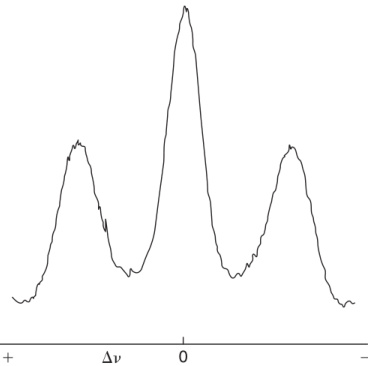
\includegraphics[width=0.33\textwidth]{images/chap15_m5c2a1bb2c993c9955e7917bd0a33b25f.jpg}
\caption{四氯化碳动力学结构因子的布里渊散射结果。}
\label{fig:15_15.10}
\end{figure}
动力学结构因子的理论表达式：
\begin{equation*}
S ( k , \omega ) = S ( k ) \left[ \left( \frac { \gamma - 1 } { \gamma } \right) \frac { 2 D _ { T } k ^{2} } { \omega ^{2} + ( D _ { T } k ^{2} ) ^{2} } + \frac { 1 } { \gamma } \left( \frac { \Gamma k ^{2} } { ( \omega ^{2} - c ^{2} k ^{2} ) ^{2} + ( \Gamma k ^{2} ) ^{2} } + \frac { \Gamma k ^{2} } { ( \omega ^{2} + c ^{2} k ^{2} ) ^{2} + ( \Gamma k ^{2} ) ^{2} } \right) \right] .
\end{equation*}

式（45）中的参数包括热扩散率\(D_{T}\)、声速\(c\)以及声衰减系数\(\Gamma\)，而\(\gamma = C_{P}/C_{V}\)则是恒压热容与恒容热容之比；参见Forster（1975）及Hansen和McDonald（1986）的相关论述。

第15.7节　翁萨格关系

大多数物理现象都表现出某种对称性，有时被称为``互易性''，这种对称性源于微观过程在宏观现象背后所具有的某些基本特性。一个显著的例子出现在不可逆过程的热力学中------在处理各种流动过程时，例如热流、电流、物质传递等。这些流动（或``电流''）是由``力''驱动的，比如温度差、电势差、压力差等，而这些力之所以发挥作用，是因为一种自然倾向。

在那些处于非平衡状态、却能逐渐接近平衡状态的物理系统中。如果系统的当前状态离平衡态并不相差太远，那么我们就可以假设力\(X_i\)与电流\(x_i\)之间存在线性关系：

\begin{equation}\tag{15.6.27}\label{eq:15.6.27}
\dot { x } _ { i } = \gamma _ { i j } X _ { j } ,
\end{equation}

其中\(\gamma_{ij}\)为系统的动力学系数。²¹ 这些系数的简单例子包括热导率、电导率、扩散系数等。然而，系统中也存在非对角元素\(\gamma_{ij}(i \neq j)\)，它们可能为零，也可能不为零；正是这些元素导致了所谓的``交叉效应''。本节所研究的内容，正是基于矩阵\(\gamma_{ij}\)的对称性特征。

解决这一问题最直观的方法，是将系统在扰动状态下的熵 \(S(x_i)\) 与其在相应平衡状态下的最大值 \(S(\tilde{x}_i)\) 进行比较。正是函数 \(S(x_i)\) 自然趋于其最大值 \(S(\tilde{x}_i)\) 的趋势，促使驱动力 \(X_i\) 被激活；这些力催生出电流 \(\tilde{x}_i\)，而这些电流则以``坐标'' \(x_i\) 为向量，将其引导至平衡态的值 \(\tilde{x}_i\)。若偏差 \((x_i - \tilde{x}_i)\) 很小，则可将函数 \(S(x_i)\) 表示为围绕 \(x_i = \tilde{x}_i\) 值展开的泰勒级数；仅保留至二阶项，我们得到：

\begin{equation}\tag{15.6.28}\label{eq:15.6.28}
\begin{array}{rl} { S ( x _ { i } ) = S ( \tilde { x } _ { i } ) + \left( \frac { \partial S } { \partial x _ { i } } \right) _ { x _ { i } = \tilde { x } _ { i } } ( x _ { i } - \tilde { x } _ { i } ) } & { } \\{ + \frac { 1 } { 2 } \left( \frac { \partial ^{2} S } { \partial x _ { i } \partial x _ { j } } \right) _ { x _ { i , j } = \tilde { x } _ { i , j } } ( x _ { i } - \tilde { x } _ { i } ) ( x _ { j } - \tilde { x } _ { j } ) . } & { } \end{array}
\end{equation}

鉴于函数 \(S(x_i)\) 在 \(x_i = \tilde{x}_i\) 处取得最大值，其一阶导数为零；因此，我们可以写出

\begin{equation}\tag{15.6.29}\label{eq:15.6.29}
\Delta S \equiv S ( x _ { i } ) - S ( \tilde { x } _ { i } ) = - \frac { 1 } { 2 } \beta _ { i j } ( x _ { i } - \tilde { x } _ { i } ) ( x _ { j } - \tilde { x } _ { j } ) ,
\end{equation}

其中

\begin{equation}\tag{15.6.30}\label{eq:15.6.30}
\beta _ { i j } = - \left( \frac { \partial ^{2} S } { \partial x _ { i } \partial x _ { j } } \right) _ { x _ { i , j } = \tilde { x } _ { i , j } } = \beta _ { j i } .
\end{equation}

驱动力 \(X_{i}\) 可以按照热力学第二定律的精神来定义，即

\begin{equation}\tag{15.6.31}\label{eq:15.6.31}
X _ { i } = \left( \frac { \partial S } { \partial x _ { i } } \right) = - \beta _ { i j } ( x _ { j } - \tilde { x } _ { j } ) .
\end{equation}

在撰写式（1）及其他后续方程时，我们遵循求和约定------该约定自动对重复的索引进行求和。

??????????????? \(X_i\) ??? \((x_i - \tilde{x}_i)\) ?????????????????????????\autoref{eq:15.1.2}?\(x_iX_j\) ????????????

\begin{equation}\tag{15.6.32}\label{eq:15.6.32}
\langle x _ { i } X _ { j } \rangle = \frac { \int _ { - \infty } ^{\infty} ( x _ { i } X _ { j } ) \exp \left\{ - \frac { 1 } { 2 k } \beta _ { i j } ( x _ { i } - \tilde { x } _ { i } ) ( x _ { j } - \tilde { x } _ { j } ) \right\} \prod _ { i } d x _ { i } } { \int _ { - \infty } ^{\infty} \exp \left\{ - \frac { 1 } { 2 k } \beta _ { i j } ( x _ { i } - \tilde { x } _ { j } ) ( x _ { j } - \tilde { x } _ { j } ) \right\} \prod _ { i } d x _ { i } } ;
\end{equation}

由于此处的积分不会因变量的较大取值而产生显著贡献，因此积分限已扩展至 \(-\infty\) 和 \(+\infty\)。同样地，

\begin{equation}\tag{15.6.33}\label{eq:15.6.33}
\langle x _ { i } \rangle = \frac { \int _ { - \infty } ^{\infty} x _ { i } \exp \left\{ - \frac { 1 } { 2 k } \beta _ { i j } ( x _ { i } - \tilde { x } _ { i } ) ( x _ { j } - \tilde { x } _ { j } ) \right\} \prod _ { i } d x _ { i } } { \int _ { - \infty } ^{\infty} \exp \left\{ - \frac { 1 } { 2 k } \beta _ { i j } ( x _ { i } - \tilde { x } _ { i } ) ( x _ { j } - \tilde { x } _ { j } ) \right\} \prod _ { i } d x _ { i } } = \tilde { x } _ { i } .
\end{equation}

对式（7）关于 \(\tilde{x}_{j}\) 求导，并牢记分母中的积分是一个常数、与各量 \(\tilde{x}_{i}\) 的实际值无关，再将所得表达式与式（6）进行比较，我们得到了一个极为重要的结论

\begin{equation}\tag{15.6.34}\label{eq:15.6.34}
\langle x _ { i } X _ { j } \rangle = - k \delta _ { i j } .
\end{equation}

接下来，我们转向论证的关键点。首先，我们注意到，尽管式（1）所讨论的是不可逆现象，但这些现象背后的微观过程却遵循时间反演法则，这意味着相关变量的时间相关性在向前或向后测量时均保持一致。因此，

\begin{equation}\tag{15.6.35}\label{eq:15.6.35}
\langle x _ { i } ( 0 ) x _ { j } ( s ) \rangle = \langle x _ { i } ( 0 ) x _ { j } ( - s ) \rangle ;
\end{equation}

此外，通过将时间的原点进行平移，

\begin{equation}\tag{15.6.36}\label{eq:15.6.36}
\langle x _ { i } ( 0 ) x _ { j } ( - s ) \rangle = \langle x _ { i } ( s ) x _ { j } ( 0 ) \rangle .
\end{equation}

将式（9）与式（10）相结合，我们得到

\begin{equation}\tag{15.6.37}\label{eq:15.6.37}
\langle x _ { i } ( 0 ) x _ { j } ( s ) \rangle = \langle x _ { i } ( s ) x _ { j } ( 0 ) \rangle .
\end{equation}

若我们从该等式的两边分别减去量 \(\langle x_{i}(0)x_{j}(0)\rangle\)，再将所得等式除以 \(s\)，并令 \(s \to 0\)，则可得

\begin{equation}\tag{15.6.38}\label{eq:15.6.38}
\langle x _ { i } ( 0 ) \dot { x } _ { j } ( 0 ) \rangle = \langle \dot { x } _ { i } ( 0 ) x _ { j } ( 0 ) \rangle .
\end{equation}

将（1）中的表达式代入，并利用（8），我们可在（12）的左侧得到

\begin{equation}\tag{15.6.39}\label{eq:15.6.39}
\langle x _ { i } ( 0 ) \gamma _ { j l } X _ { l } ( 0 ) \rangle = - k \gamma _ { j l } \delta _ { i l } = - k \gamma _ { j i }
\end{equation}

而在其右侧

\begin{equation}\tag{15.6.40}\label{eq:15.6.40}
\langle \gamma _ { i l } X _ { l } ( 0 ) x _ { j } ( 0 ) \rangle = - k \gamma _ { i l } \delta _ { j l } = - k \gamma _ { i j } .
\end{equation}

由此可知，

\begin{equation}\tag{15.6.41}\label{eq:15.6.41}
\gamma _ { i j } = \gamma _ { j i } .
\end{equation}

方程（13）构成了翁萨格互易关系；这些关系最早由翁萨格于1931年推导出来，并已成为不可逆现象热力学中不可或缺的一部分。

鉴于方程（1）和方程（13），电流 \(\dot{x}_{i}\) 可写为

\begin{equation}\tag{15.6.42}\label{eq:15.6.42}
\dot { x } _ { i } = \frac { \partial f } { \partial X _ { i } } ,
\end{equation}

其中，生成函数 \(f\) 是力 \(X_i\) 的二次函数：

\begin{equation}\tag{15.6.43}\label{eq:15.6.43}
f = \frac { 1 } { 2 } \gamma _ { i j } X _ { i } X _ { j } .
\end{equation}

函数 \(f\) 至关重要，因为它直接决定了系统熵随时间变化的速率：

\begin{equation}\tag{15.6.44}\label{eq:15.6.44}
\dot { S } = \frac { \partial S } { \partial x _ { i } } \dot { x } _ { i } = X _ { i } \dot { x } _ { i } = X _ { i } \frac { \partial f } { \partial X _ { i } } = 2 f .
\end{equation}

当系统接近平衡态时，其熵必将向平衡值 \(S(\tilde{x}_i)\) 增加。因此，函数 \(f\) 必须为正定函数，这为系数 \(\gamma_{ij}\) 带来了若干限制条件。

与方程（1）类似，我们同样可以写出

\begin{equation}\tag{15.6.45}\label{eq:15.6.45}
\dot { X } _ { i } = \zeta _ { i j } ( x _ { j } - \tilde { x } _ { j } ) ,
\end{equation}

量 \(\zeta_{ij}\) 则是与系统相关的另一组系数。另一方面，根据方程（1）和方程（5），我们得到

\begin{equation}\tag{15.6.46}\label{eq:15.6.46}
\begin{array}{rl} & { \dot { X } _ { i } = - \beta _ { i j } \dot { x } _ { j } = - \beta _ { i j } ( \gamma _ { j l } X _ { l } ) = - \beta _ { i j } \gamma _ { j l } \{ - \beta _ { l m } ( x _ { m } - \tilde { x } _ { m } ) \} } \\& { = \beta _ { i j } \gamma _ { j l } \beta _ { l m } ( x _ { m } - \tilde { x } _ { m } ) . } \end{array}
\end{equation}

将方程（17）与方程（18）进行比较，我们得以得出新系数 \(\zeta_{ij}\) 与动力学系数 \(\gamma_{ij}\) 之间的关系：

\begin{equation}\tag{15.6.47}\label{eq:15.6.47}
\zeta _ { i m } = \beta _ { i j } \gamma _ { j l } \beta _ { l m } .
\end{equation}

现在，鉴于矩阵 \(\beta\) 和 \(\gamma\) 的对称性，我们得到

\begin{equation}\tag{15.6.48}\label{eq:15.6.48}
\zeta _ { i m } = \zeta _ { m i } ;
\end{equation}

因此，通过现象学方程（17）引入的系数 \(\zeta_{ij}\) 也遵循互易关系。由此可知，量 \(\dot{X}_{l}\) 可以表示为，

\begin{equation}\tag{15.6.49}\label{eq:15.6.49}
\dot { X } _ { i } = \frac { \partial f ^{\prime} } { \partial x _ { i } } ,
\end{equation}

其中

\begin{equation}\tag{15.6.50}\label{eq:15.6.50}
f ^{\prime} = \frac { 1 } { 2 } \zeta _ { i j } ( x _ { i } - \tilde { x } _ { i } ) ( x _ { j } - \tilde { x } _ { j } ) .
\end{equation}

熵的变化 \(dS\) 现可表示为

\begin{equation}\tag{15.6.51}\label{eq:15.6.51}
\begin{array}{rl} & { d S = \frac { \partial S } { \partial x _ { j } } d x _ { j } = X _ { j } d x _ { j } = - \beta _ { j i } ( x _ { i } - \tilde { x } _ { i } ) d x _ { j } } \\& {  = ( x _ { i } - \tilde { x } _ { i } ) d \{ - \beta _ { i j } ( x _ { j } - \tilde { x } _ { j } ) \} = ( x _ { i } - \tilde { x } _ { i } ) d X _ { i } , } \end{array}
\end{equation}

从而

\begin{equation}\tag{15.6.52}\label{eq:15.6.52}
\frac { \partial S } { \partial X _ { i } } = ( x _ { i } - \tilde { x } _ { i } ) ;
\end{equation}

显然，熵 \(S\) 现在被视为力 \(X_i\) 的显式函数（而非坐标 \(x_i\) 的函数）。而 \(S\) 的时间导数现变为

\begin{equation}\tag{15.6.53}\label{eq:15.6.53}
\dot { S } = \frac { \partial S } { \partial X _ { i } } \dot { X } _ { i } = ( x _ { i } - \tilde { x } _ { i } ) \frac { \partial f ^{\prime} } { \partial X _ { i } } = 2 f ^{\prime} .
\end{equation}

通过比较式（16）与式（25），我们得出结论：函数 \(f\) 与 \(f'\) 实际上是相同的；它们只是以两种不同的变量集来表示而已。

在此有必要指出，翁萨格的互易关系与前一节中的涨落-耗散定理有着密切的联系。根据式（15.6.18）和式（15.6.19），并采用求和约定，在当前的上下文中，

\begin{equation}\tag{15.6.54}\label{eq:15.6.54}
\dot { x } _ { i } ( t ) = \frac { 1 } { k T } \int _ { - \infty } ^{t} E _ { l } ( t ^{\prime} ) \langle \dot { x } _ { l } ( t ^{\prime} ) \dot { x } _ { i } ( t ) \rangle d t ^{\prime}
\end{equation}

或者，令 \((t-t')=s\)，

\begin{equation}\tag{15.6.55}\label{eq:15.6.55}
\dot { x } _ { i } ( t ) = \frac { 1 } { k T } \int _ { 0 } ^{\infty} E _ { l } ( t - s ) \langle \dot { x } _ { l } ( t - s ) \langle \dot { x } _ { i } ( t ) \rangle d s ;
\end{equation}

将此与式（1）进行对比。交换指标 \(i\) 和 \(l\)，我们得到

\begin{equation}\tag{15.6.56}\label{eq:15.6.56}
\dot { x } _ { l } ( t ) = \frac { 1 } { k T } \int _ { 0 } ^{\infty} E _ { i } ( t - s ) \langle \dot { x } _ { i } ( t - s ) \dot { x } _ { l } ( t ) \rangle d s .
\end{equation}

如今的关键在于，式（27）和式（28）中出现的相关函数在数值上完全相同，对于

\begin{equation}\tag{15.6.57}\label{eq:15.6.57}
\langle \dot { x } _ { l } ( t - s ) \dot { x } _ { i } ( t ) \rangle = \langle \dot { x } _ { l } ( 0 ) \dot { x } _ { i } ( s ) \rangle = \langle \dot { x } _ { l } ( 0 ) \dot { x } _ { i } ( - s ) \rangle = \langle \dot { x } _ { l } ( t ) \dot { x } _ { i } ( t - s ) \rangle ;
\end{equation}

在推导式（29）时，第一步和第三步源于``时间的平移''，而第二步则源自``微观过程的动力学可逆性原理''。式（29）所展现的等价关系，本质上正是翁萨格互易关系的内涵。尤其是，如果式（27）和式（28）中出现的相关函数在 \(s=0\) 的值处呈现出尖峰状分布，则这些方程将退化为现象学方程（1），而式（29）也将与翁萨格关系（13）同义。

最后，我们对关系（13）作一些进一步的说明。我们回顾一下，在推导这些关系的过程中，我们不得不借助微观过程在时间反演下的不变性。然而，对于``旋转系统''（或``处于外加磁场中的系统''）而言，情况则略有不同：在这种情况下，微观过程在时间反演下的不变性只有在角速度 \(\Omega\)（或磁场 \(B\)）同时发生符号反转时才成立。此时，那些可能依赖于参数 \(\Omega\)（或 \(B\)）的动力学系数，将满足以下关系：

\begin{equation}\tag{15.6.58}\label{eq:15.6.58}
\gamma _ { i j } ( \Omega ) = \gamma _ { j i } ( - \Omega )
\end{equation}

并且

\begin{equation}\tag{15.6.59}\label{eq:15.6.59}
\gamma _ { i j } ( \pmb { B } ) = \gamma _ { j i } ( - \pmb { B } ) .
\end{equation}

此外，我们的证明还建立在这样一个隐含假设之上：量 \(x_{i}\) 本身在时间反演下不会发生变化。若出于某种原因，这些量与某一宏观运动的速度成正比，那么它们在时间反演下也会改变符号。现在，如果 \(x_{i}\) 和 \(x_{j}\) 都属于这一类，那么对我们的证明至关重要的式（12）将保持不变；因此，系数 \(\gamma_{ij}\) 和 \(\gamma_{ji}\) 仍将相等。然而，如果其中仅有一者属于这一类，而另一者不属于，则式（12）将变为

\begin{equation}\tag{15.6.60}\label{eq:15.6.60}
\langle x _ { i } ( 0 ) \dot { x } _ { j } ( 0 ) \rangle = - \langle \dot { x } _ { i } ( 0 ) x _ { j } ( 0 ) \rangle ;
\end{equation}

此时，系数 \(\gamma_{ij}\) 和 \(\gamma_{ji}\) 将满足以下关系：

\begin{equation}\tag{15.6.61}\label{eq:15.6.61}
\gamma _ { i j } = - \gamma _ { j i } .
\end{equation}

在将翁萨格关系应用于不同物理问题时，可参考德·格鲁特（1951年）、德·格鲁特与马祖尔（1962年）以及普里戈金（1967年）所著的专著。

\section{问题}\label{ux95eeux9898_chap15}

15.1. ??\autoref{eq:15.1.11}?\autoref{eq:15.1.12}?? \(\Delta S\) ? \(\Delta P\)????\autoref{eq:15.1.14}?? \(\overline{(\Delta T)^2}\)?\(\overline{(\Delta V)^2}\) ?? \(\overline{(\Delta T\Delta V)}\)????

\begin{enumerate}
\def\labelenumi{(\alph{enumi})}
\item
  \(\overline{(\Delta T \Delta S)} = kT\)；(b) \(\overline{(\Delta P \Delta V)} = -kT\)；
\item
  \(\overline{(\Delta S \Delta V)} = kT(\partial V / \partial T)_{P}\)；(d) \(\overline{(\Delta P \Delta T)} = kT^{2} C_{V}^{-1} (\partial P / \partial T)_{V}\)。
\end{enumerate}

请注意，结果 (a) 和 (b) 可写为：\((\Delta T\Delta S - \Delta P\Delta V) = 2kT\)，这一结果直接源于概率分布函数 (15.1.8)。

15.2. ??????\autoref{eq:15.1.15}????????\autoref{eq:15.1.16}??? \((\Delta S)^2\)?\((\Delta P)^2\) ? \((\Delta S\Delta P)\) ????????????????????????????????

15.3. ????? \(E\) ? \(V\) ???????????????? \autoref{eq:15.1.8} ???????\autoref{eq:15.1.13}?\autoref{eq:15.1.15}??????????????????? \(\Delta E \Delta V\) ?????????????\(E\) ? \(V\) ?????????\((\Delta E \Delta V) \neq 0\)?

因此，\(E\) 和 \(V\) 并非统计上独立的：\(\overline{(\Delta E \Delta V)} \neq 0\)。请证明：

\begin{equation}\tag{15.6.62}\label{eq:15.6.62}
\overline { { ( \Delta E \Delta V ) } } = k T \left\{ T \left( \frac { \partial V } { \partial T } \right) _ { P } + P \left( \frac { \partial V } { \partial P } \right) _ { T } \right\} ;
\end{equation}

????\autoref{eq:15.1.14}?\autoref{eq:15.1.18}??? \(\overline{(\Delta V)^2}\) ? \(\overline{(\Delta E)^2}\) ?????

{[}请注意，在二维正态分布的情况下，即

\begin{equation}\tag{15.6.63}\label{eq:15.6.63}
p ( x , y ) \propto \exp \left\{ - \frac { 1 } { 2 } ( a x ^{2} + 2 b x y + c y ^{2} ) \right\} ,
\end{equation}

量 \(\langle x^{2}\rangle\)、\(\langle x y\rangle\) 和 \(\langle y^{2}\rangle\) 可以通过对公式进行对数求导来轻松得到。

\begin{equation}\tag{15.6.64}\label{eq:15.6.64}
\int _ { - \infty } ^{\infty}    \int _ { - \infty } ^{\infty} \exp \left\{ - { \frac { 1 } { 2 } } ( a x ^{2} + 2 b x y + c y ^{2} \right\} d x \, d y = { \frac { 2 \pi } { \sqrt { ( a c - b ^{2} ) } } }
\end{equation}

对参数 \(a\)、\(b\) 和 \(c\) 进行求导。由此可得该分布的协方差矩阵，即

\begin{equation}\tag{15.6.65}\label{eq:15.6.65}
\begin{pmatrix}\langle x^2\rangle&\langle xy\rangle\\\langle yx\rangle&\langle y^2\rangle\end{pmatrix}=\frac1{(ac-b^2)}\begin{pmatrix}c&-b\\-b&a\end{pmatrix}.
\end{equation}

若 \(b=0\)，则

\begin{equation}\tag{15.6.66}\label{eq:15.6.66}
\langle x ^{2} \rangle = 1 / a ,  \langle x y \rangle = 0 ,  \langle y ^{2} \rangle = 1 / c . ] ^{22}
\end{equation}

15.4. 一根长度为 \(l\) 的绳子在恒定张力 \(F\) 的作用下，被拉伸于两个固定点 \(A\) 和 \(B\) 之间。请证明，位于距离 \(A\) 为 \(x\) 的点 \(P\) 处的平均平方（涨落）位移 \(y(x)\) 可以表示为

\begin{equation}\tag{15.6.67}\label{eq:15.6.67}
\overline { { \{ y ( x ) \} ^{2} } } = \frac { k T } { F l } x ( l - x ) .
\end{equation}

\(^{22}\)关于\(n\)维正态分布的协方差矩阵，请参阅兰道与利夫希茨（1958），第110节。

进一步证明，对于\(x_{2} \geq x_{1}\)，

\begin{equation}\tag{15.6.68}\label{eq:15.6.68}
\overline { { y ( x _ { 1 } ) y ( x _ { 2 } ) } } = \frac { k T } { F l } x _ { 1 } ( l - x _ { 2 } ) .
\end{equation}

【提示】：计算与所讨论的涨落相关的能量\(\Phi\)；随后，所需的概率分布由\(p \propto \exp(-\Phi/kT)\)给出，由此可轻松求得所需的各种平均值。

15.5. 在常温常压下，一个气相子系统的体积\(V_A\)必须有多小，才能使占据该体积的粒子数\(N_A\)的均方根偏差达到平均值\(\overline{N_A}\)的1\%？

15.6. 波斯皮希尔（1927）观察到了直径为\(0.4 \times 10^{-4}\)厘米的烟尘颗粒在水-甘油溶液中的布朗运动，该溶液的粘度为0.0278泊，温度为18.8°C。在10秒的时间间隔内，观测到的\(\overline{x}^2\)值为\(3.3 \times 10^{-8}\)平方厘米。利用这些数据，求出玻尔兹曼常数\(k\)。

15.7. ??15.3?? notation ???????????????

\begin{equation}\tag{15.6.69}\label{eq:15.6.69}
\langle \pmb { v } ( t ) \cdot \pmb { F } ( t ) \rangle = 3 k T / \tau ,  \mathrm { w h i l e } \; \; \langle \pmb { v } ( t ) \cdot \pmb { \mathcal { F } } ( t ) \rangle = 0 .
\end{equation}

另一方面，

\begin{equation}\tag{15.6.70}\label{eq:15.6.70}
\langle \pmb { r } ( t ) \cdot \mathcal { F } ( t ) \rangle = - 3 k T ,  \mathrm { w h i l e } \; \; \langle \pmb { r } ( t ) \cdot \pmb { F } ( t ) \rangle = 0 .
\end{equation}

15.8. ?\autoref{eq:15.3.14}????????

\begin{equation}\tag{15.6.71}\label{eq:15.6.71}
\pmb { r } ( t ) = \pmb { v } ( 0 ) \tau ( 1 - e ^{- t / \tau} ) + \tau \int _ { 0 } ^{t} \{ 1 - e ^{( u - t ) / \tau} \} \pmb { A } ( u ) d u ,
\end{equation}

??\(r(0)=0\)???????????????????\(K_{\mathrm{A}}(s)\)???????\(\langle r^{2}(t)\rangle\)????15.3.31??

15.9. 在使用动圈式检流计探测极其微弱的电流时，必须确保观测到的偏转并非仅仅由于悬浮系统布朗运动产生的偶然扰动所致。如果我们认为，偏转角\(\theta\)的大小超过\(4\theta_{\mathrm{r.m.s.}}[=4(kT/c)^{1/2}]\)，则这种偏转极不可能是布朗运动造成的，从而我们可以得出一个下限，即通过该检流计能够可靠记录的电流强度。将这一极限电流用时间周期\(\tau\)和检流计的临界阻尼电阻\(R_{c}\)来表示。

15.10. ?a??????\(v_{x}\)???????\autoref{eq:15.3.5}??????\(\delta t\)?????????

\begin{equation}\tag{15.6.72}\label{eq:15.6.72}
\frac { \langle \delta v _ { x } \rangle } { \delta t } = - \frac { v _ { x } } { \tau }  \mathrm { a n d }  \frac { \langle ( \delta v _ { x } ) ^{2} \rangle } { \delta t } = \frac { 2 k T } { M \tau } .
\end{equation}

（b）现在，建立福克-普朗克方程，用于描述分布函数\(f(\nu_x,t)\)，并结合前述关于\(\mu_1(\nu_x)\)和\(\mu_2(\nu_x)\)的结果，推导出该函数的显式表达式。深入研究各种具有重要意义的情形，尤其是当\(t \gg \tau\)的情况。

15.11. ??\autoref{eq:15.3.33}?????????????????????????????????? \(t=0\) ??????? \(x(0)\)?????? \(\nu(0)\)??????????? \(\langle x^2(t) \rangle\) ? \(\langle v^2(t) \rangle\) ????????? \(\omega_0 \to 0\) ?????????????\autoref{eq:15.3.29}?\autoref{eq:15.3.31}??? \(M \to 0\) ?????????? 15.4 ???????

15.12. 将福克-普朗克方程推广至粒子在三维空间中进行布朗运动的情形。求解该方程的一般解，并研究其重要特征。

15.13. 某一统计平稳变量 \(y(t)\) 的自相关函数 \(K(s)\) 可以表示为：（a）\(K(s) = K(0)e^{-\alpha s^2}\cos(2\pi f^*s)\)，或

（b）\(K(s) = K(0)e^{-\alpha|s|}\cos(2\pi f^*s)\)，

其中 \(\alpha > 0\)。分别确定并讨论上述两种情形下功率谱 \(w(f)\) 的性质，并探究其在以下极限下的行为：（a）\(\alpha \to 0\)，（b）\(f^* \to 0\)，以及（c）\(\alpha\) 和 \(f^*\) 都趋于零。

15.14. 证明：若某一统计平稳变量 \(y(t)\) 的自相关函数 \(K(s)\) 可以表示为

\begin{equation}\tag{15.6.73}\label{eq:15.6.73}
K ( s ) = K ( 0 ) \frac { \sin ( a s ) } { a s } \frac { \sin ( b s ) } { b s }  ( a > b > 0 ) ,
\end{equation}

则该变量的功率谱 \(w(f)\) 可以表示为

\begin{equation}\tag{15.6.74}\label{eq:15.6.74}
\begin{array}{rlrl} & { w ( f ) = \frac { 2 \pi } { a } K ( 0 ) } & & { \mathrm { f o r ~ } 0 < f \leq \frac { a - b } { 2 \pi } , } \\& { \frac { 2 \pi } { a b } K ( 0 ) \left\{ \frac { a + b } { 2 } - \pi f \right\} } & & { \mathrm { f o r ~ } \frac { a - b } { 2 \pi } \leq f \leq \frac { a + b } { 2 \pi } , } \\& { 0 } & & { \mathrm { f o r ~ } \frac { a + b } { 2 \pi } \leq f < \infty . } \end{array}
\end{equation}

???? \(w(f)\) ??????15.5.16?????

????? \(b \to 0\) ???????????????15.5.18????????

（a）证明，由公式定义的变量 \(Y(t)\) 的均方值为

\begin{equation}\tag{15.6.75}\label{eq:15.6.75}
Y ( t ) = \int _ { u } ^{u + t} y ( u ) d u ,
\end{equation}

其中 \(y(u)\) 是具有功率谱 \(w(f)\) 的统计平稳变量，其值为

\begin{equation}\tag{15.6.76}\label{eq:15.6.76}
\langle Y ^{2} ( t ) \rangle = \frac { 1 } { 2 \pi ^{2} } \int _ { 0 } ^{\infty} \frac { w ( f ) } { f ^{2} } \left\{ 1 - \cos ( 2 \pi f t ) \right\} d f ;
\end{equation}

相应地，

\begin{equation}\tag{15.6.77}\label{eq:15.6.77}
\begin{array}{r} { w ( f ) = 4 \pi f \int _ { 0 } ^{\infty} \frac { \partial } { \partial t } \langle Y ^{2} ( t ) \rangle \sin ( 2 \pi f t ) d t } \\{ = 2 \int _ { 0 } ^{\infty} \frac { \partial ^{2} } { \partial t ^{2} } \langle Y ^{2} ( t ) \rangle \cos ( 2 \pi f t ) d t . } \end{array}
\end{equation}

?????????? MacDonald?1962??? 2.2.1 ??????????15.5.14??????????

\begin{equation}\tag{15.6.78}\label{eq:15.6.78}
K _ { \gamma } ( s ) = \frac { 1 } { 2 } \frac { \partial ^{2} } { \partial s ^{2} } \langle Y ^{2} ( s ) \rangle .
\end{equation}

（b）将前述分析应用于布朗运动粒子的运动，将 \(y\) 定义为粒子的速度，而 \(Y\) 则为粒子的位移。

15.16. ????????????\autoref{eq:15.3.5}?????? \(\nu(t)\) ? \(A(t)\) ???? \(w_{\nu}(f)\) ? \(w_{A}(f)\) ?????????

\begin{equation}\tag{15.6.79}\label{eq:15.6.79}
w _ { v } ( f ) = w _ { A } ( f ) \frac { \tau ^{2} } { 1 + ( 2 \pi f \tau ) ^{2} } ,
\end{equation}

\(\tau\) ?????????????????15.5.21??\(w_{A}(f) = \frac{12kT}{M\tau}\)?

15.17. ?a???\autoref{eq:15.6.7}?\autoref{eq:15.6.9}?

\begin{enumerate}
\def\labelenumi{(\alph{enumi})}
\setcounter{enumi}{1}
\tightlist
\item
?\autoref{eq:15.6.9}?? \(K_{\nu}(s)\) ???\autoref{eq:15.6.6}??????????????? \(\langle r^{2}(t)\rangle\) ?\autoref{eq:15.3.31}?
\end{enumerate}

15.18. 确定在谐振子势场中布朗粒子的 \(\hat{\chi}_{vx}''(\omega)\) 和 \(S_{vx}(\omega)\)。证明，在这种情况下，响应函数与功率谱之间存在联系，且这一关系可由涨落-耗散定理的经典极限来解释。

15.19. ????\autoref{eq:15.6.28}??????????? \autoref{eq:15.6.29}?

15.20. ?? \(G_{AB}(t) = G_{BA}(t - i\beta\hbar)\)????????????????-?????\(\hat{\chi}_{AB}^{\prime\prime}(\omega) = \frac{1}{2\hbar} \left(1 - e^{-\beta\hbar\omega}\right)S_{AB}(\omega)\)?

15.21. ?? \(G_{AB}(t) = G_{BA}(t - i\beta\hbar)\)?????????????????\(\hat{\chi}_{AB}^{\prime\prime}(t)\) ?? \(\left\langle\frac{dA(t)}{dt}B(0)\right\rangle\)???????????\autoref{eq:15.6.39}????

15.22. ?\autoref{eq:15.6.41}????????????????????????????? \(S_{\mathrm{self}}(\boldsymbol{k},\omega)\) ??????????????????? \(\langle e^{f}\rangle = \exp\left(\langle f^{2}/2\rangle\right)\)?

15.23. 使用波长 \(\lambda = 632.8\) nm 的 He-Ne 激光，确定水分子中 90° 激光散射 Brillouin 峰的角频率 \(\omega_{k}\)。确定 Rayleigh 峰的宽度，并证明 Brillouin 峰与 Rayleigh 峰之间具有良好的分离度。水的热扩散系数为 \(D_{T} = 1.4 \times 10^{-7}\,\mathrm{m}^{2}/\mathrm{s}\)。

15.24. 描述以波长 \(\lambda = 632.8\) nm 的 He-Ne 激光为光源的拉曼散射的动力学结构因子。负责该散射的能量能级为 0.05 eV，该能级的寿命为 1 皮秒。在室温下，当 \(\omega \to -\omega\) 时，斯托克斯散射与反斯托克斯散射是否对称？


